%%%%%%%%%%%%%%%%%%%%%%%%%%%%%%%%%%%%%%%%%%%%%%%%%%%%%%%%%%%%%%%%%%%%%%%%%%%%%%%%
%Objetivo: Descrever os principais conceitos relativos a Manutenção de Software
%		   envolvidos na dissertação
%Autores: Vagner Clementino <vagnercs@dcc.ufmg.br>
%		  Rodolfo Resende <rodolfo@dcc.ufmg.br>
%Criação: Ter Set 13 19:22:37 BRT 2016
%Modificação: sex mai  5 13:17:17 UTC 2017
%Revisão: sáb mai 27 17:13:26 -03 2017
%%%%%%%%%%%%%%%%%%%%%%%%%%%%%%%%%%%%%%%%%%%%%%%%%%%%%%%%%%%%%%%%%%%%%%%%%%%%%%%%

\chapter{As FGRMs no Contexto da Manutenção de Software}
\label{ch:visao-geral-manutencao}

A tendência é que os sistemas de software evoluam para atender aos requisitos e
alterações do ambiente no qual eles estejam inseridos. Em uma série de estudos,
Lehman propôs leis sobre a evolução do software. A Lei da Mudança Contínua
(Continuing Change) afirma que um software em uso deve mudar ou se tornará
progressivamente menos útil~\cite{lehman1980understanding}. A Lei da
Complexidade Crescente (Increasing complexity) afirma que as mudanças realizadas
em um sistema torna a sua estrutura cada vez mais complexa. Neste contexto,
recursos extras devem ser disponibilizados a fim de preservar e simplificar a
estrutura do software~\cite{lehman1980understanding}. As leis de Lehman têm sido
validadas, especialmente aquelas relacionadas ao tamanho e complexidade do
software. Em um trabalho sobre o tema Yu \& Mishra~\cite{{yu2013empirical}}
examinaram de forma empírica as Leis de Lehman em relação a evolução da
qualidade do software. O estudo demonstrou que a qualidade de um produto de
software declinará a menos que uma restruturação seja realizada.

Partindo da premissa de que mudanças em software são inevitáveis, torna-se
importante uma disciplina com foco no gerenciamento e controle das alterações.
Em geral, dentro do escopo da Engenharia de Software a tarefa fica a cargo da
\textit{Manutenção de Software}. Nas próximas seções discutiremos os conceitos
básicos da Manutenção de Software que foram utilizados nesta dissertação e sua
relação com as FGRMs, que é a sigla para Ferramentas de Gerenciamento de
Requisições de Mudança que é o software utilizado para gerenciar uma Requisição
de Mudança, o veículo de comunicação de uma falha ou melhoria entre as
diferentes partes interessadas de um projeto de software.

\section{A Manutenção de Software e a Requisição de Mudança}
\label{sec:conceitos_basicos}

Nesta seção apresentamos terminologias que ajudam no entendimento do papel e
finalidade da Manutenção de Software e a relação destes termos com o conceito de
Requisição de Mudança. Iniciaremos com uma visão geral do processo de Manutenção
de Software.

\subsection{Visão Geral da Manutenção de Software}
\label{sub:visão_geral_da_manutenção_de_softare}

De uma maneira geral, podemos definir a atividade de manter software como a
totalidade das ações necessárias para fornecer suporte a um produto de software.
No Padrão IEEE 1219~\cite{ISO-1219-1998} ela é definida como a modificação de um
produto de software após a sua entrega com o objetivo de corrigir falhas,
melhorar o desempenho ou outros atributos com a finalidade de adaptar o sistema
às modificações ambientais.

Posteriormente a IEEE/EIA 12207~-~Padrão para o Processo de Ciclo de Vida do
Software~\cite{ISOIEC-12207-2008}, retrata a manutenção como um dos principais
processos no ciclo de vida do software. Em seu texto a disciplina é definida
como a atividade de modificação do código e da documentação associada em
decorrência de uma falha ou necessidade de melhoria no
software~\cite{IEEEComputerSociety:2014:GSE:2616205}.

De maneira relacionada, \textit{Manutenibilidade} é a propriedade de um sistema
ou componente de software em relação ao grau de \textit{facilidade} que ele pode
ser corrigido, melhorado ou adaptado~\cite{{159342}}. A
ISO/IEC~9126~-~01~\cite{ISOIEC9126} define a Manutenibilidade como um atributo
de qualidade do processo de Manutenção.

É possível verificar que  \textit{manter e evoluir} são aspectos comuns das
diferentes definições para Manutenção de Software. Embora exista o entendimento
que os processos de manutenção e evolução possuem características
distintas~\cite{tripathy2014software}, não está nos objetivos desta dissertação
discutir e apresentar as diferenças. Neste sentido, utilizamos ambos os termos
de forma intercambiáveis.

%A Manutenção é necessária para garantir que o software seja capaz de satisfazer
%os requisitos dos usuários. Neste sentido, a atividade de manter software pode
%ser vista como um desenvolvimento contínuo, sobretudo, pelo fato que alguns
%sistemas nunca estão completos e continuam a evoluir.

\subsection{O Processo de Manutenção de Software}
\label{sec:o_processo_de_manutecao_de_software}

O Processo de Manutenção de Software é o conjunto de atividades, métodos,
práticas e transformações utilizadas para desenvolver ou manter um software e
seus artefatos associados~\cite{paulk1993key}. Existe na literatura alguns
modelos para o processo de manutenção de software, especialmente baseados em uma
visão ``tradicional''. Nesta perspectiva o desenvolvimento e a manutenção de
software possuem uma separação clara. Contudo, no momento do desenvolvimento
desta dissertação, existia uma tendência de adoção das práticas propostas pelos
agilistas na manutenção de software. Esta inclinação surge da demanda por
serviços de manutenção de rápido retorno para o usuário.

%Nas próximas seções apresentamos alguns modelos encontrados na literatura na
%perspectiva tradicional, ao mesmo tempo descrevemos propostas do uso da
%metodologia dos agilistas na manutenção de software.

\subsubsection{Manutenção de Software Tradicional}
\label{subsec:manutenção_de_software_tradicional}

Nesta seção apresentamos e discutimos alguns modelos para o processo de
manutenção, que segundo o nosso entendimento, são os principais disponíveis na
literatura. No contexto desta dissertação estes modelos são descritos como
tradicionais. Em resumo, um processo de manutenção de software descreve as
atividades e suas respectivas entradas e saídas. Alguns modelos são descritos
nos padrões IEEE 1219 e ISO/IEC 14764. O processo especificado no padrão
IEEE\@-\@1219 indica que as atividades de manutenção de software iniciem após a
entrega do produto de software. O padrão também discute aspectos de planejamento
da manutenção. As atividades que compõem o processo são apresentadas na
Figura~\ref{fig:ieee-1219-processo-man-software}.

\begin{figure}[htpb] \centering
	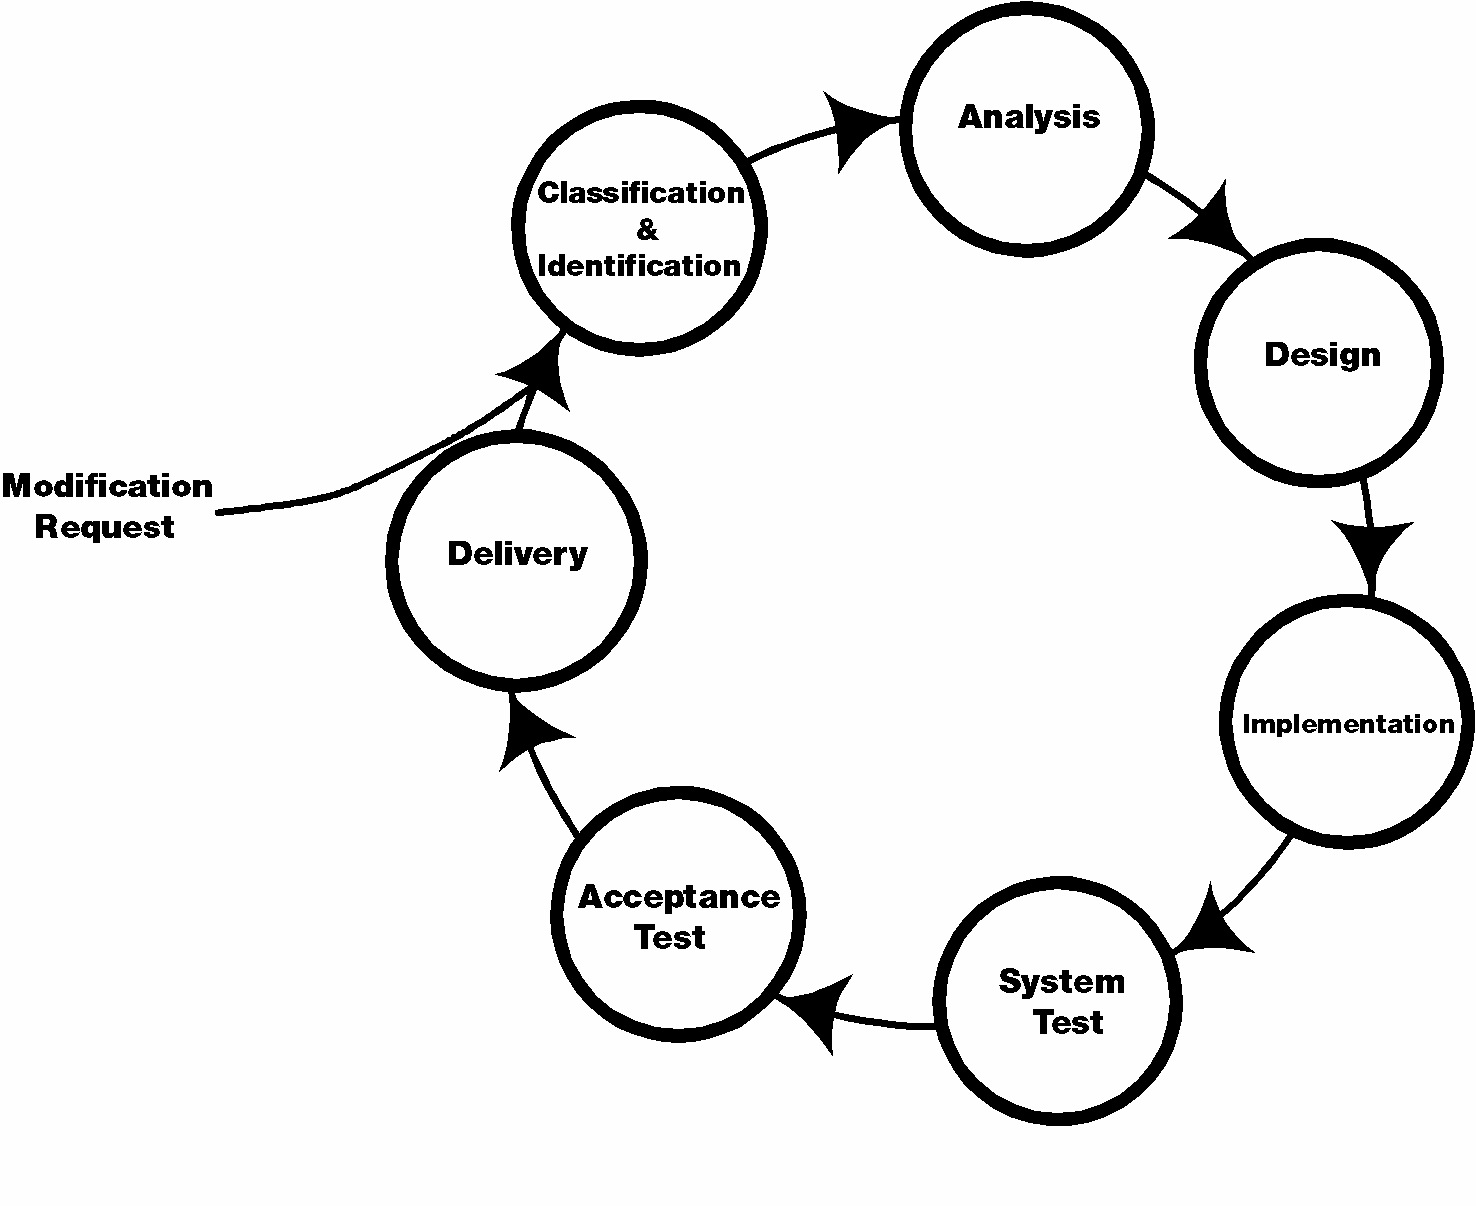
\includegraphics[width=0.5\linewidth]{./chapter-manutencao-software-visao-geral/img/ieee_1219_98_processo_manutencao.png}
	\caption{IEEE 1219 -~Processo de Manutenção de
		Software}\label{fig:ieee-1219-processo-man-software}
\end{figure}

De maneira relacionada, na ISO/IEC 14764 as atividades que compõem o processo
são similares aquelas propostas na IEEE-~1219, exceto pelo fato que elas são
agregadas de uma forma diferente. O processo descrito na ISO/IEC~14764 são
exibidas na Figura~\ref{fig:ieee-14764-processo-manutencao}.

\begin{figure}[htpb] \centering
	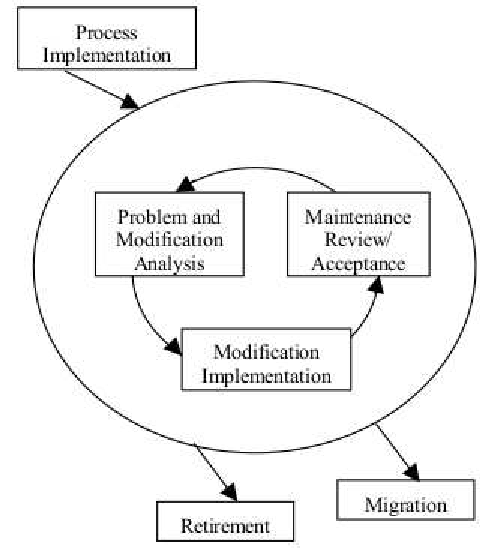
\includegraphics[width=0.5\linewidth]
{chapter-manutencao-software-visao-geral/img/ieee-14764-processo-manutencao.pdf}
	\caption{ISO/IEC~14764 Processo de Manutenção de Software}
\label{fig:ieee-14764-processo-manutencao} \end{figure}

As atividades de manutenção propostas na ISO/IEC 14764 são detalhadas nas
tarefas descritas a seguir:

\begin{itemize}
   	\item Implementação do Processo
   	\item Análise e Modificação do
		Problema
	\item Aceitação e Revisão da Manutenção
   	\item Migração
   	\item Aposentadoria do Software
\end{itemize}

É possível notar que algumas atividades realizadas durante a manutenção de
software são similares a outras presentes no desenvolvimento de software, como
por exemplo, análise de desempenho, codificação, teste e documentação. Outra
atividade comum à manter e desenvolver software é o gerenciamento dos
requisitos. Nas duas situações os profissionais responsáveis por controlar os
requisitos devem atualizar a do\-cu\-men\-ta\-ção  por conta de alterações
ocorridas no código fonte. Por outro lado, certas atividades estão vinculadas
apenas ao contexto da manutenção de software. O Corpo de Conhecimento em
Engenharia de Software~\cite{4425813} destaca algumas delas:

\begin{description}
	\item[Compreensão do programa:] atividades necessárias para obter um
		conhecimento geral do que um produto de software faz e como as partes
		funcionam em conjunto;
    \item[Transição:] uma sequência controlada e coordenada de atividades em que
        o software é transferido progressivamente do desenvolvedor para o
        mantenedor;
    \item[Aceitação/rejeição de Requisições de Mudança:] as modificações que
        ultrapassem determinado limiar de tamanho, esforço ou complexidade podem
        ser rejeitadas pelos mantenedores e redirecionadas para outro
        desenvolvedor;
	\item[Suporte ao usuário:] uma função de suporte para o usuário final que
		pode resultar na priorização ou avaliação de esforço das Requisições
		de Mudança;
	\item[Análise de impacto:] uma técnica para identificar os módulos que
		possivelmente são afetados por determinada mudança solicitada;
	\item[Contratos de Acordo de Nível de Serviço (Service Level Agreements
		\@-\@ SLA):] acordos contratuais que descrevem os serviços a serem
		realizados pela equipe de manutenção e os objetivos de qualidade do
		produto de software.
\end{description}

\subsubsection{Manutenção de Software na Perspectiva dos Agilistas}
\label{sub:manutenção_de_software_com_método_dos_agilistas}

Grande parte da literatura em Manutenção de Software trata de técnicas e
metodologias tradicionais da Engenharia de Software. Todavia, verifica-se a
tendência de que os departamentos dedicados à Manutenção de Software se mostrem
interessados nas metodologias propostas pelos agilistas~\cite{Heeager2015}.  No
momento da elaboração desta dissertação boa parte dos textos em Engenharia de
Software tratam desenvolvimento e manutenção como atividades com natureza
distintas. Todavia, algumas ``práticas ágeis'' podem ser utilizadas em tarefas
de manutenção tais como processo de trabalho iterativo, um maior envolvimento do
cliente, a comunicação face a face e os testes frequentes.

A adoção das práticas dos agilistas na manutenção de software pode apresentar
algumas dificuldades~\cite{1402140}. Entre elas está a adequação das práticas da
organização com as necessidades do time de desenvolvimento. Por outro lado, no
trabalho de Choudhari \& Suman~\cite{Choudhari:2014:EIM:2557833.2557845} que
propõe um modelo de processo para manutenção de software usando práticas da
Programação Extrema (Extreme Programming \@-\@ XP), apresenta como resultado:
melhorias no aprendizado e produtividade da equipe por meio do aumento da moral,
encorajamento e confiança entre os desenvolvedores.

\subsection{Papéis na Manutenção de Software}
\label{subsec:man_visao_geral_papeis_na_manutencao_de_software}

As ações realizadas durante a manutenção de um software são desempenhadas por
diferentes pessoas. Neste processo cada integrante da equipe de manutenção pode
desempenhar um ou mais papéis. Os nomes e as atividades desenvolvidas por cada
um pode variar de um projeto para outro, contudo, é possível determinar uma
classificação que agregue um ponto comum entre os diferentes papéis. Nesta
dissertação, utilizamos a classificação proposta por Polo e
outros~\cite{Polo1999} cujo objetivo é definir a estrutura da equipe de
manutenção através da identificação das tarefas que cada membro deve executar.
O conjunto de papéis é o resultado da aplicação da metodologia
MANTEMA~\cite{756695} em projetos de software bancários espanhóis em que o setor
de manutenção foi terceirizado (outsourcing). Os autores reforçam que apesar da
classificação ter sido criada em um contexto específico, ela pode ser utilizada para
aplicação em outras situações.

Para esta dissertação removemos os papéis que segundo o nosso entendimento estão
mais vinculados a um contexto de manutenção terceirizada (outsourcing).  Além
disso, dividimos o papel ``time de manutenção' (maintenance team) em
\textit{Desenvolvedor e Analista de Qualidade} por entendermos que são
atribuições comuns a muito dos processos de manutenção existentes. Os papéis que
compõem a classificação utilizadas durante o texto da dissertação estão
descritos a seguir:

\paragraph{Usuário Afetado:}
Indivíduo que utiliza o sistema do qual pertence à Requisição de Mudanças (RM)
que será relatada. O defeito, a melhoria ou evolução no software, representada
pela RM, estão relacionadas com os desejos e necessidades deste papel.

\paragraph{Reportador:}
Responsável por registrar a RM que pode ser qualquer pessoa envolvida no
processo de Manutenção de Software. Neste sentido, as atividades relacionadas
com o papel de Reportador podem estar vinculados com outras contidas nesta
classificação. A Figura~\ref{fig:diagrama-caso-uso-reportador} apresenta esta
situação através de um Diagrama de Caso de Uso, em que o \textit{Reportador} pode
ser um usuário do sistema ou um membro da equipe de manutenção.

\begin{figure}[htpb]
	\centering
	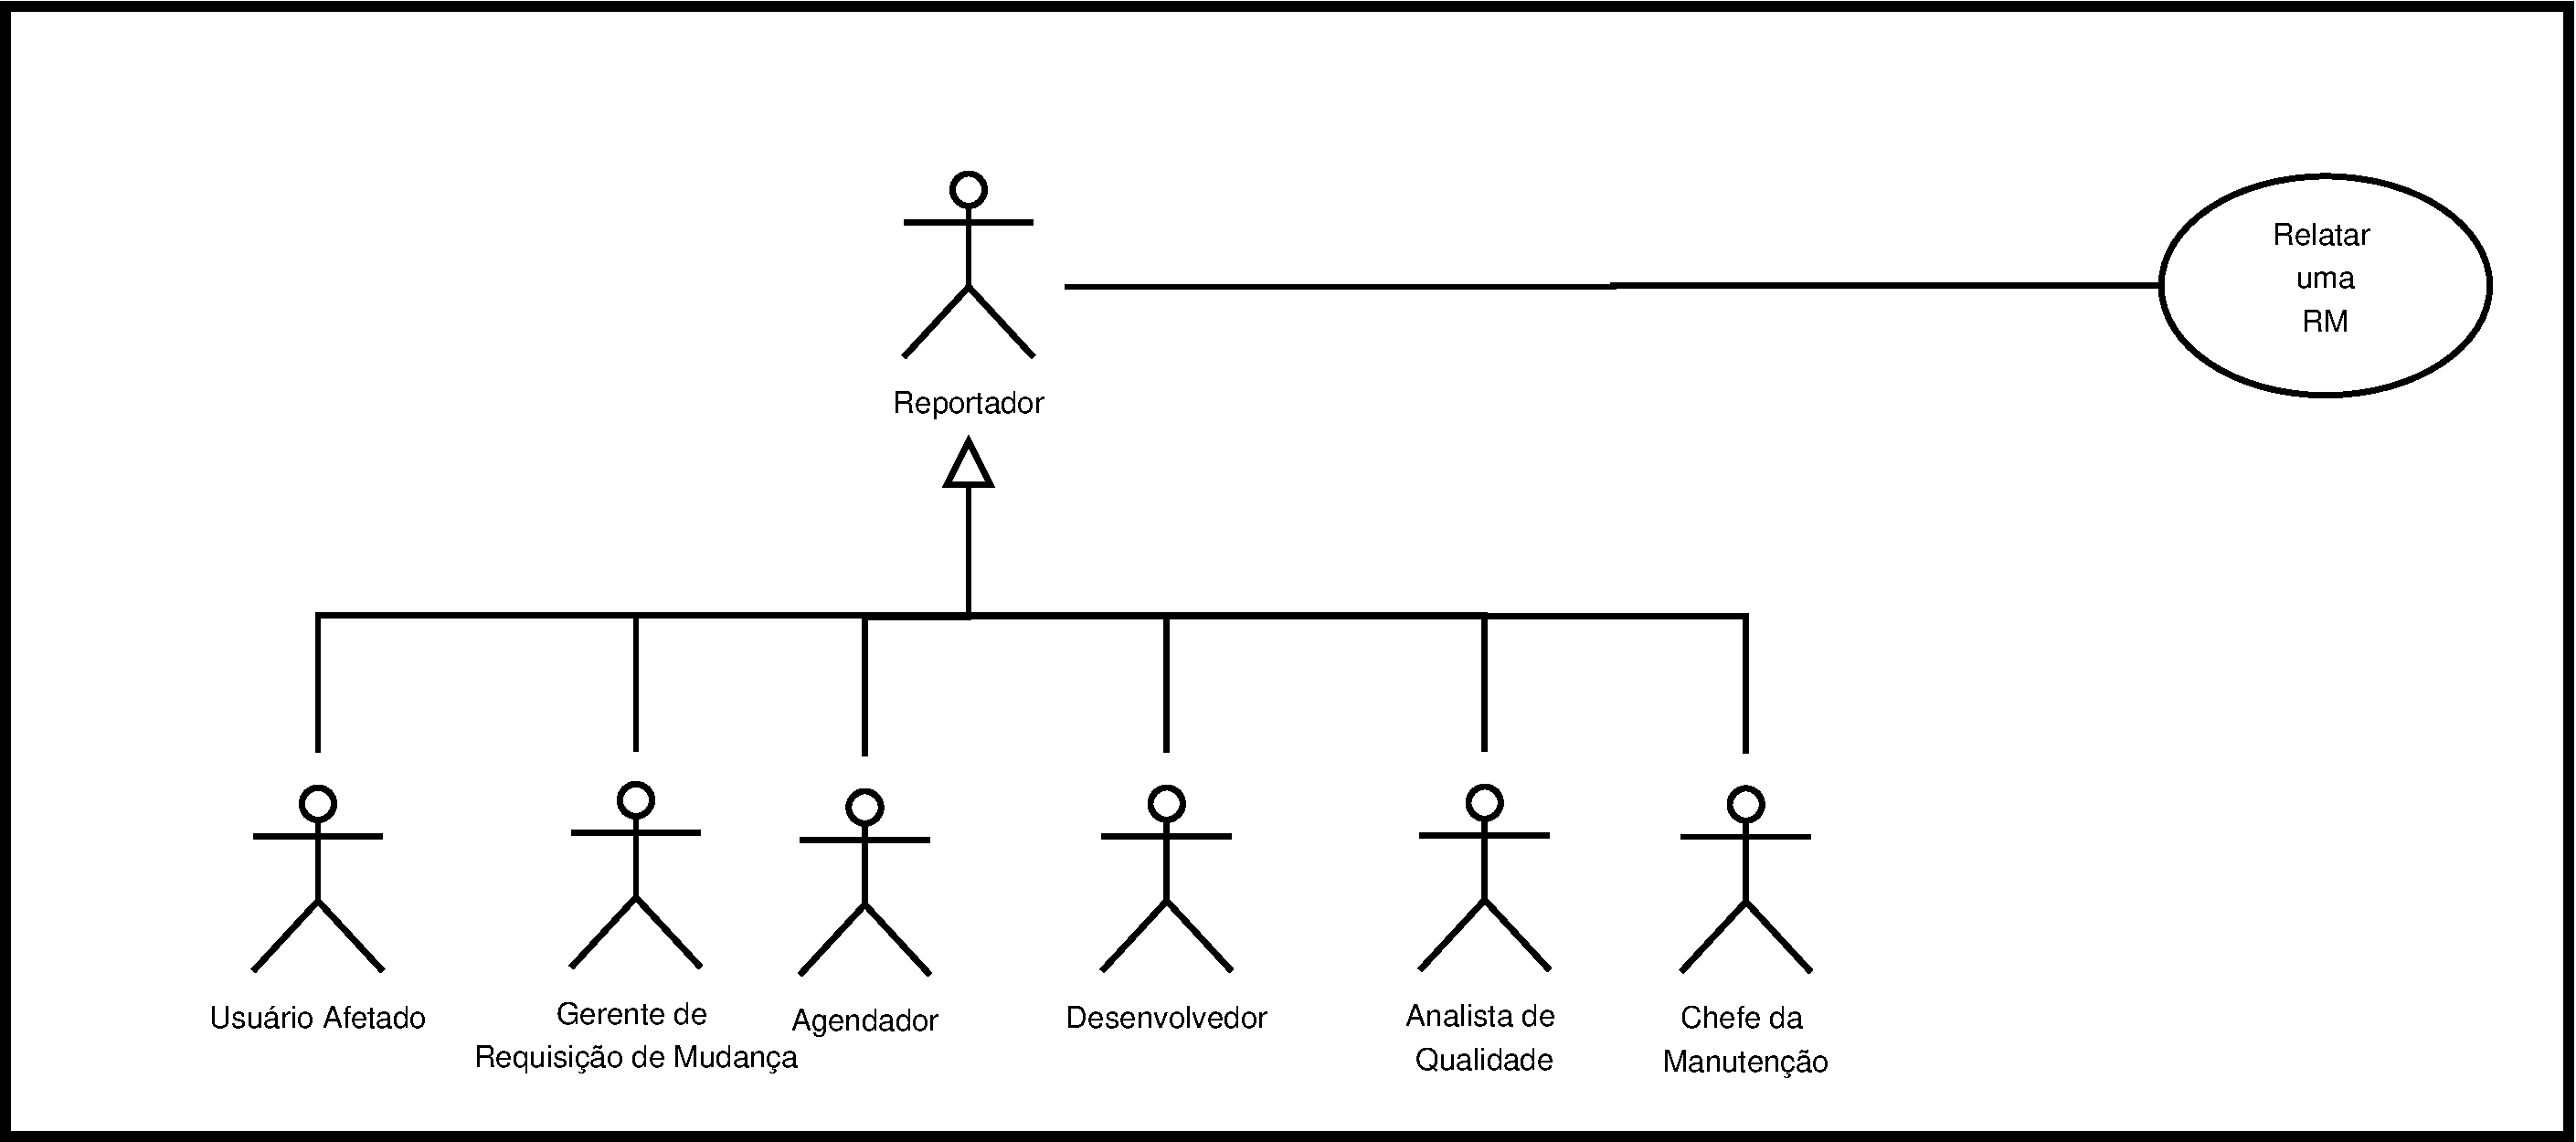
\includegraphics[width=0.8\linewidth]{./chapter-manutencao-software-visao-geral/img/diagrama-caso-uso-reportador.pdf}
	\caption{Diagrama de caso de uso do papel Reportador}
\label{fig:diagrama-caso-uso-reportador}
\end{figure}

\paragraph{Gerente de Requisição de Mudança (Maintenance-request manager):}
Res\-pon\-sá\-vel por decidir se uma RM será aceita ou rejeitada. Além disso,
ele define qual tipo de manutenção deverá ser aplicada. Posteriormente cabe a
este profissional encaminhar a RM para o Agente de Triagem.

\paragraph{Agente de Triagem (Scheduler)}:
Deve planejar a fila de RMs e atribuí-las para o desenvolvedor mais apto. A
decisão pode considerar a carga de trabalho existente para cada possível
destinatário da RM\@.

\paragraph{Desenvolvedor:}
Responsável por realizar as ações que irão solucionar a RM\@.

\paragraph{Analista de Qualidade:}
Tem por responsabilidade avaliar se uma RM solucionada por um Desenvolvedor foi
resolvida de forma correta e dentro dos padrões de qualidade exigidos pelo
projeto.

\paragraph{Chefe da Manutenção (Head of	Maintenance):}
Este papel é responsável por definir os padrões e procedimentos que compõem o
processo de manutenção que será utilizado.

Apesar da classificação de papéis derivar de um contexto específico (setor
bancário e empresas com a área de manutenção terceirizada), ela é capaz de
acoplar com tipos modelos de processo de manutenção existente na literatura. Um
exemplo está no trabalho proposto por Ihara e
outros~\cite{Ihara:2009:AMI:1595808.1595833} em que foi criada uma representação
de um processo de modificação de falhas (bugs) tomando como base as diversas
estágios de uma RM no contexto de projetos de código aberto. O processo
resultante é facilmente acoplável com a classificação proposta por Polo e outros
e que utilizada nesta dissertação.

Cabe ressaltar que está fora do escopo deste estudo elaborar uma classificação dos
papeis envolvidos na Manutenção de Software em função de supormos que isto
corresponde a um esforço bem extenso. Nossa ação é identificar se existem papeis
e quais são eles, sem com isso, envolver em uma consolidação definitiva.

\subsection{Requisição de Mudança}
\label{sec:requisicao_de_mudanca}

\subsubsection{Conceitos Básicos}
\label{subsec:tipos_de_requisicoes_mudanca}

%As manutenções em software podem ser divididas em \textit{Corretiva,
%Adaptativa, Perfectiva e Preventiva}~\cite{Lientz:1980:SMM:601062,159342}.  A
%Manutenção Corretiva lida com a reparação de falhas encontradas. A Adaptativa
%tem o foco na adequação do software devido à mudanças ocorridas no ambiente em
%que ele está inserido. A Perfectiva trabalha para detectar e corrigir falhas
%latentes. A Preventiva preocupa com atividades que possibilitem aumento da
%manutenibilidade do sistema.  A ISO 14764~\cite{1703974} propõe a divisão da
%tarefa de manutenção nos quatro tipos descritos anteriormente e propõe que
%exista um elemento comum denominado Requisição de Mudança (RM) que representa
%as características comuns a todas aqueles tipos de manutenção. A
%Figura~\ref{fig:modification-request} exibe a classificação das RMs conforme
%discutido pela ISO\@.


%A ISO/IEC 14764 classifica as manutenções adaptativas e perfectivas como
%me\-lho\-ri\-as e agrupa as manutenções corretivas e preventivas em uma única
%categoria de correção, conforme exibido na
%Tabela~\ref{tab:categorias_requisicao_mudanca}. A manutenção preventiva é
%frequentemente realizada em produtos de software em que atributos de segurança são
%mais críticos.

%\begin{table}[htpb] \centering 	\begin{tabular}{l|l|l|} \cline{2-3} &
		%\textbf{Correção} & \textbf{Melhoria} \\ \hline
		%\multicolumn{1}{|l|}{\textbf{Pró-ativa}} & Preventiva & Perfectiva \\
		%\hline \multicolumn{1}{|l|}{\textbf{Reativa}} & Corretiva & Adaptativa
		%\\ \hline \end{tabular}\caption{Categorias da Requisição de Mudanças.
		%Adaptado de
		%SWEBOK~\cite{4425813}}\label{tab:categorias_requisicao_mudanca}
%\end{table}

%Alguns pesquisadores e profissionais entendem a manutenção preventiva como um
%subconjunto da perfectiva~\cite{tripathy2014software}.

Uma Requisição de Mudança (RM) é o veículo para registrar a informação sobre o
defeito, evolução ou melhoria de um sistema~\cite{tripathy2014software}. De
maneira geral, uma RM pode ser especializada como o \textit{Pedido de Correção}
de uma falha ou o \textit{Pedido de Melhoria} que pode estar relacionado com o
aprimoramento de funcionalidades ou com a melhoria da qualidade do sistema. Esta
visão é apresentada na Figura~\ref{fig:diagrama-classe-requisicao-mudancas}.
Alguns autores utilizam os termos \textit{relato de defeito ou relato de
    melhoria} como sinônimos para a RM\@. Todavia, no escopo desta dissertação,
o relato é um atributo da RM que representa o texto que descreve uma falha ou
pedido de melhoria (vide
Figura~\ref{fig:diagrama-classe-atributos-requisicao-mudancas}).

\begin{figure}[htpb]
	\centering
	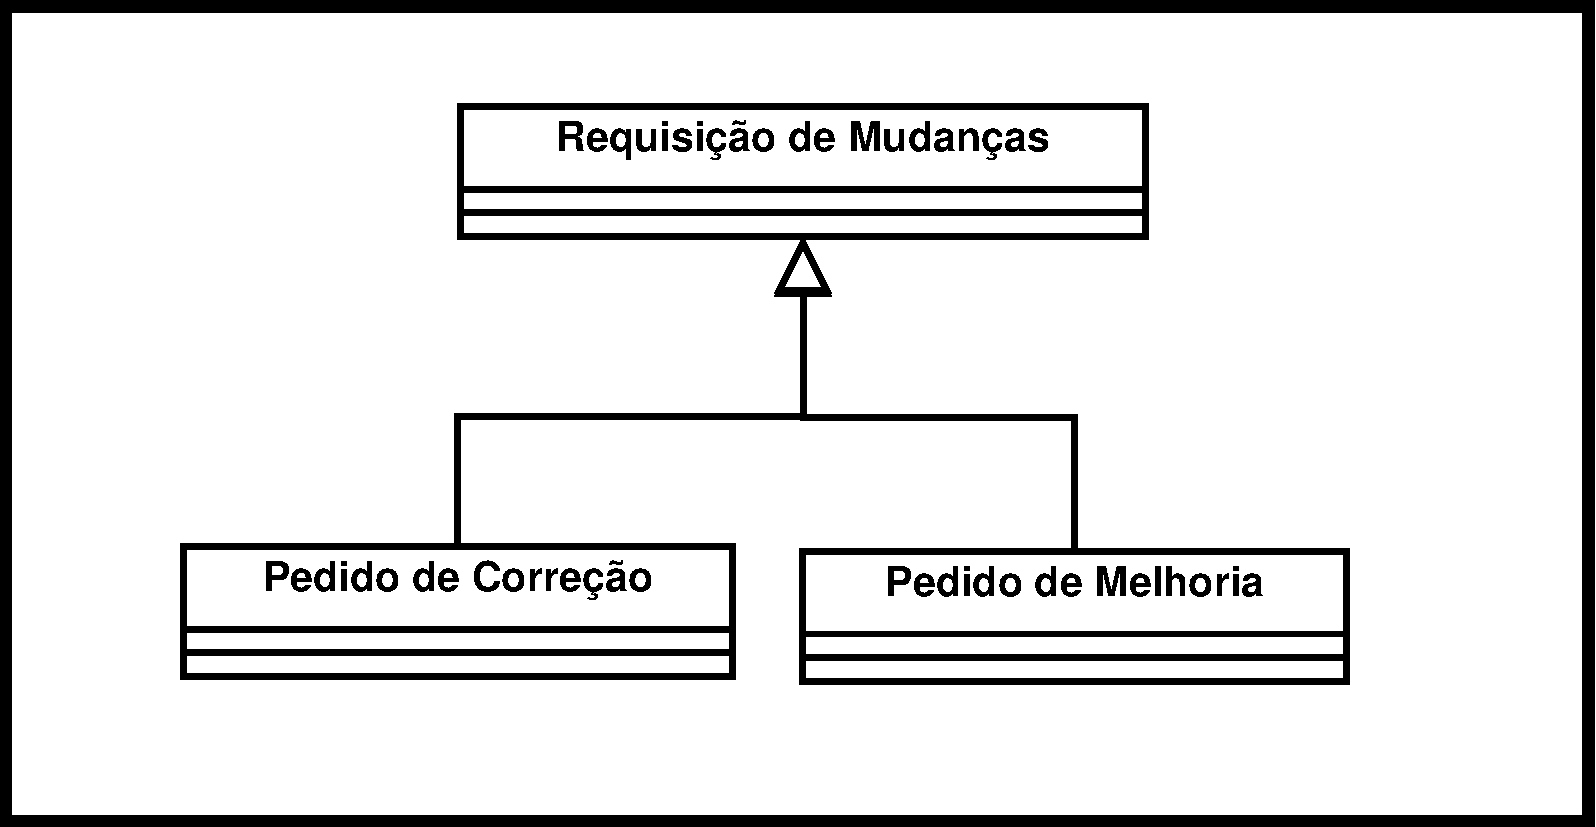
\includegraphics[width=0.5\linewidth]{./chapter-manutencao-software-visao-geral/img/diagrama-classe-conceitual-requisicao-mudancas.pdf}
	\caption{Modelo conceitual de uma Requisição de Mudanças}
\label{fig:diagrama-classe-requisicao-mudancas}
\end{figure}

As principais características que compõem uma RM podem ser visualizadas no
modelo exibido na
Figura~\ref{fig:diagrama-classe-atributos-requisicao-mudancas}. Trata-se de uma
adaptação do que foi proposto no trabalho de Singh \&
Chaturvedi~\cite{singh2011bug} que descreve um processo genérico de como uma RM
é relatada.

\begin{figure}[htpb]
	\centering
	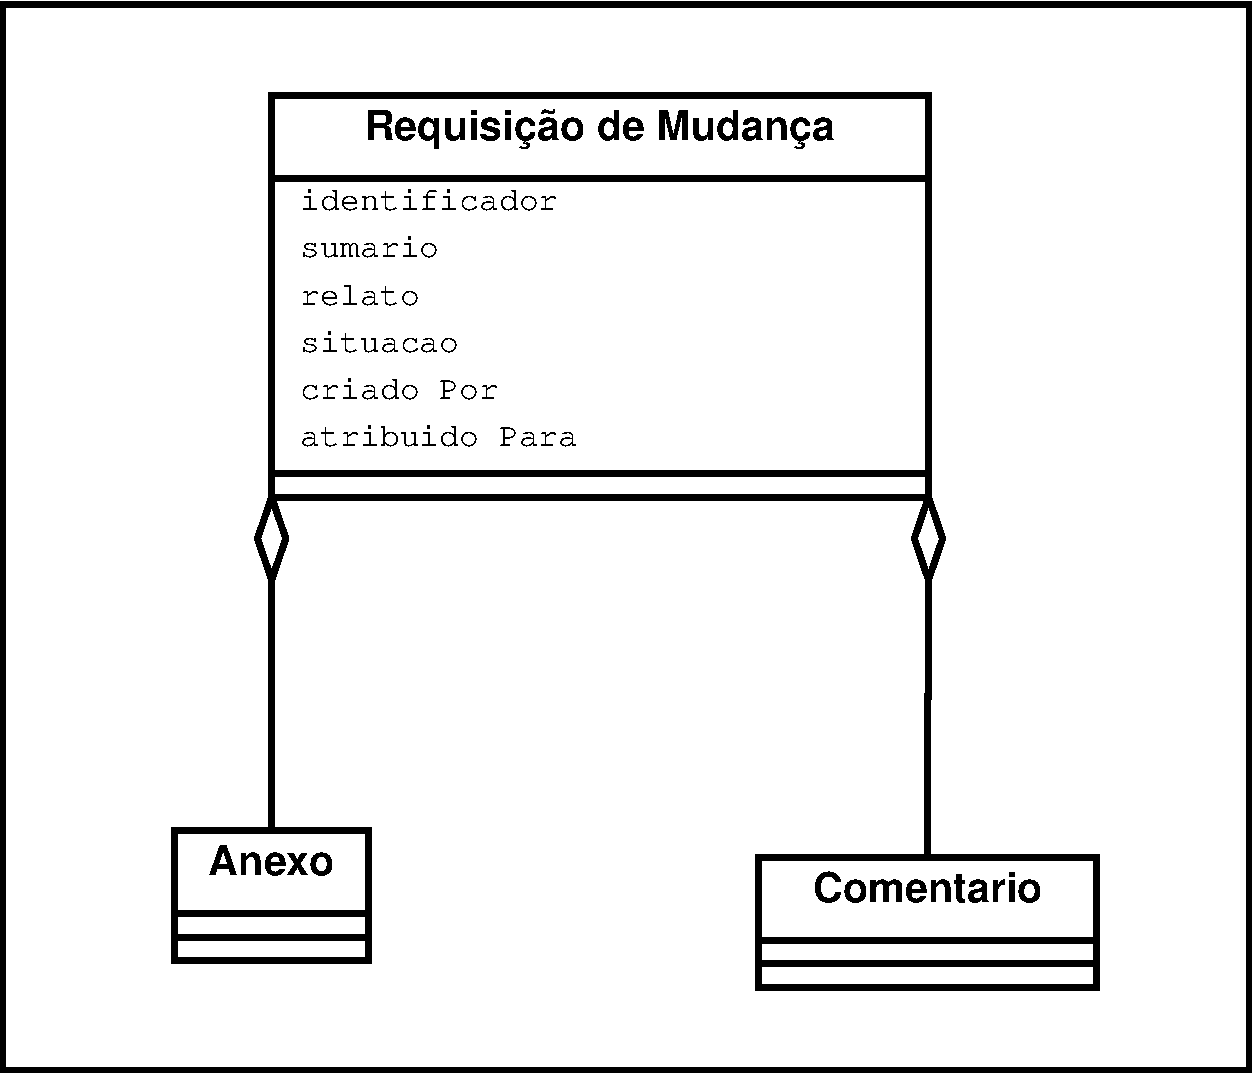
\includegraphics[width=0.5\linewidth]{./chapter-manutencao-software-visao-geral/img/diagrama-classe-atributos-requisicao-mudancas.pdf}
	\caption{Informações que compõem uma RM}
\label{fig:diagrama-classe-atributos-requisicao-mudancas}
\end{figure}

Os principais conceitos envolvidos no modelo estão detalhados a seguir:

\begin{description}
    \item [Identificador] Sequência de caracteres, geralmente numérica,  que
        permite distinguir de maneira única uma RM\@.
	\item [Sumário] Um título ou resumo da RM\@.
    \item [Relato] Descrição detalhada da RM incluindo ``o que'', ``onde'',
        ``por quê'', ``como'' e ``quando'' a situação relatada ocorreu. A
        mensagem que aparece durante a operação do sistema pode ser incluída,
        bem como a entrada inserida e/ou a saída esperada.
	\item [Situação] A situação atual de uma RM\@. Representa os diversos
		estados que uma RM possui em seu ciclo de vida. Nesta dissertação
		discutimos brevemente o ciclo de vida de uma RM na
		Subseção~\ref{sub:fluxo_de_trabalho_requisicao_mudanca}.
    \item [Criado Por] Nome da pessoa ou um identificador previamente registrado
        no sistema de quem criou a RM\@.
    \item [Atribuído Para] A RM pode ser atribuída a uma pessoa específica caso
        ela seja capaz de resolvê-la, caso contrário, a RM será atribuída para
        alguém que possui o papel de definir o desenvolvedor mais apto para
        solucioná-la. Neste estudo, o membro de uma equipe de manutenção com
        esta função é denominado \textit{Agente de Triagem}.
    \item [Anexo] Refere-se a informação em formato diferente de texto e que
        pode ser incluída na RM\@. Por exemplo, casos de teste, capturas de
        tela, e cadeia de registros de ativação (stack trace).
    \item [Comentário] Registra o histórico de discussões realizadas durante o
        processo de solução da RM\@\footnote{O conceito de solução bem como de
            outros relacionados ao ciclo de vida de uma RM estão descritos com
        maiores detalhes na Seção~\ref{sub:fluxo_de_trabalho_requisicao_mudanca}}.
\end{description}

Conforme pode ser observado na
Figura~\ref{fig:diagrama-classe-atributos-requisicao-mudancas} os atributos
\textit{Comentário} e \textit{Anexo} foram modelados como uma agregação, dando
aos mesmos um caráter multi-valorado. Esta escolha foi intencional para salientar
que uma RM pode conter diversos anexos ou comentários. No caso dos comentários
esta característica é ainda mais relevante tendo em vista que eles são
realizados durante o processo de solução de uma RM\@. A partir do conjunto de
comentários é possível coletar informações relevantes para a manutenção do
software e que podem ser utilizadas para solucionar futuras RMs.

Os atributos que compõem uma RM pode variar dependendo de fatores como a
ferramenta utilizada para o gerenciamento, o projeto e a equipe de manutenção.
Esses campos fornecem uma variedade de metadados descritivos tais como
\textit{importância, prioridade, gravidade, componente, e
    produto}~\cite{zhang2016literature}. Em alguns casos a RM pode conter um
campo de modo à relacioná-la com outra já existente na base de dados. Este tipo
de vínculo é importante para minimizar problemas da gestão das RMs como por
exemplo as duplicadas. Alguns dos problemas relacionados com a gestão das RMs
estão descritos na Seção~\ref{ssub:problemas_relacionadas_rm}. A
Figura~\ref{fig:rm-exemplo} exibe um exemplo representativo de uma RM contendo
os elementos básicos descritos no modelo proposto na
Figura~\ref{fig:diagrama-classe-atributos-requisicao-mudancas}.

\begin{figure}[htpb]
	\centering
	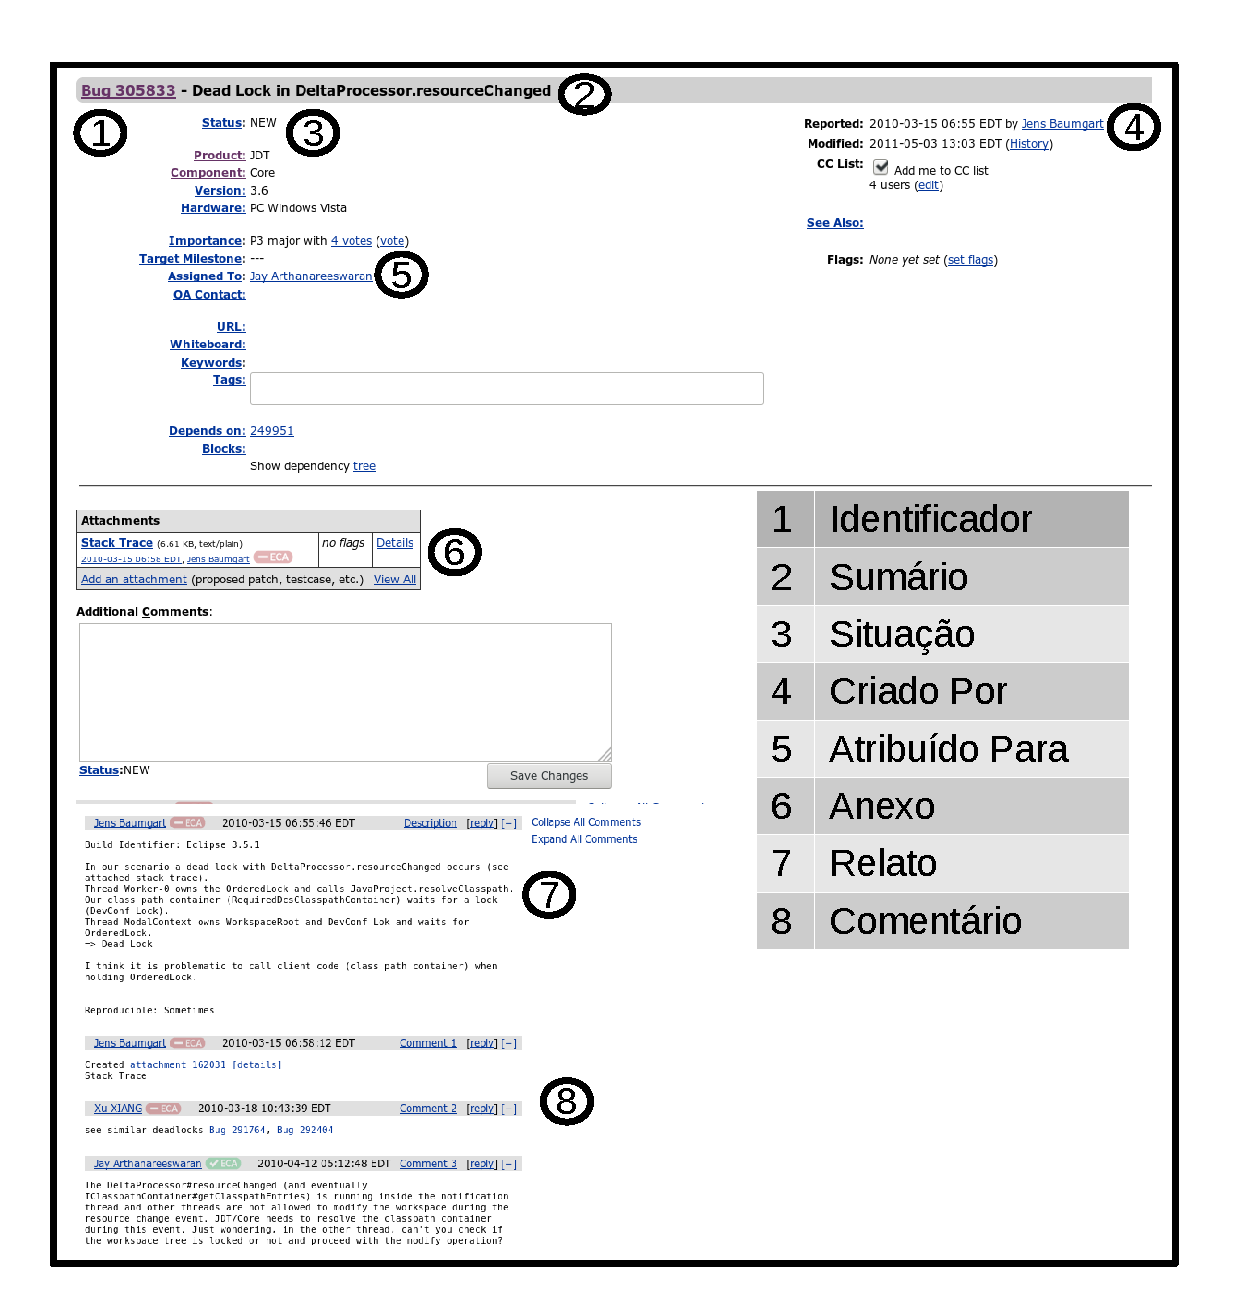
\includegraphics[width=0.8\linewidth]{./chapter-manutencao-software-visao-geral/img/rm-exemplo.pdf}
	\caption{Um exemplo de uma RM do Projeto Eclipse}
\label{fig:rm-exemplo}
\end{figure}

Em síntese, apesar das diferentes nomenclaturas existentes na literatura
(demanda, bug, defeito, bilhete, tíquete, requisição de modificação, relato de
problema) uma Requisição de Mudança representa uma descrição, independente da
estrutura, que visa gerar a manutenção ou evolução do software. A manutenção ou
evolução estão relacionados com o reparo de uma falha ou com um desejo ou
necessidade do usuário do software. Nesta dissertação procuramos ficar aderentes
ao termo ``Requisição de Mudança'' e sua sigla \textit{RM}.

\subsubsection{Ciclo de Vida de uma Requisição de Mudança}
\label{sub:fluxo_de_trabalho_requisicao_mudanca}

Uma RM descreve os desejos e necessidades dos usuários de como um sistema deve
operar. Quando uma RM é relatada dois fatores devem ser levados em
conta~\cite{tripathy2014software}:

\begin{itemize}
	\item \textit{Corretude da RM:} uma RM deve ser descrita de forma não
		ambígua tal que seja fácil revisá-la afim de determinar sua corretude. O
		``formulário'', que são os campos que devem ser preenchidos na RM, são a
		chave para efetiva interação entre a organização que desenvolve o
		software e os seus usuários. O formulário, neste sentido, documenta
		informações essenciais sobre mudanças no software, hardware e
		documentação.
   \item \textit{Comunicação clara das RMs entre as partes
           interessadas\footnote{Na
               Seção~\ref{subsec:man_visao_geral_papeis_na_manutencao_de_software}
               discutiremos em maior detalhe as diferentes partes interessadas
               no contexto da manutenção de software.}}: as RMs necessitam ser
       claramente comunicadas entre as parte interessadas, inclusive entre a
       equipe de manutenção. O resultado de avaliar de maneira distinta uma RM
       pode ser contra-produtivo: \textit{(i)} a equipe que realiza mudanças no
       sistema e a equipe que executa testes podem ter visões contraditórias
       sobre a qualidade do software; \textit{(ii)} O sistema alterado pode não
       atender às necessidades e desejos dos usuários finais.
\end{itemize}

No caminho entre sua criação e solução uma RM possui diferentes estágios. O
ciclo de vida de uma RM é ilustrado através do diagrama de estados da
Figura~\ref{fig:diagrama-estado-rm}. Nele uma RM inicia como \textit{Submetida
    (Submit)} e vai sendo modificada até alcançar o estado \textit{Fechada
    (Closed)}, em que é considerada como solucionada. Neste caminho o conjunto
de fatores que resultou na necessidade de relatar a RM pode não mais existir.
Neste caso, ela é alterada para o estado \textit{Rejeitada (Decline)}.

Existe um aspecto importante do ciclo de vida de uma RM que não consta na
discussão apresentada por Tripathy \& Naik. Em teoria uma RM poderia ter novos
estados: ``Reaberta'', quando um usuário ou outro membro da equipe de manutenção
entende que ela não foi solucionada; ``Relacionada'', quando uma nova RM é na
realidade uma sucessora ou possui algum tipo de relação com outra RM
anteriormente registrada.

\begin{figure}[htpb]
	\centering
	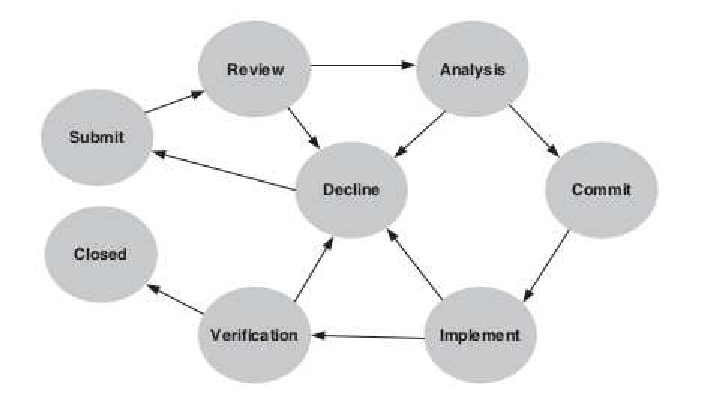
\includegraphics[width=0.5\linewidth]{./chapter-manutencao-software-visao-geral/img/diagrama-estado-rm.pdf}
	\caption{Diagrama de estados de uma RM\@. Extraído
		de~\cite{tripathy2014software}}
\label{fig:diagrama-estado-rm}
\end{figure}

A seguir apresentamos as características dos estados do ciclo de vida de uma
RM\@ como base na discussão realizada por Tripathy \&
Naik~\cite{tripathy2014software}. Para cada estado pode haver mais de um papel
responsável pelas ações executadas. Também pode ocorrer que uma mesma pessoa
desempenhe diferentes papéis neste processo. Uma discussão sobre os papéis
utilizados no escopo desta dissertação pode ser encontrada na
Seção~\ref{subsec:man_visao_geral_papeis_na_manutencao_de_software}.

\paragraph{Submetida (Submit).}
\label{par:submetida)}

Este é o estado inicial de uma RM criada. Geralmente são os usuários do sistema
a fonte primária das RMs nesta situação. Com base no nível de prioridade, ela é
movida de \textit{Submetida} para \textit{Em Revisão}. Normalmente cabe ao
\textit{Gerente de Requisição de Mudança} a responsabilidade da manipulação
inicial das RMs. Neste instante ele se torna o ``dono'' das mesmas.

\paragraph{Em Revisão (Review).}
\label{par:em_revisao}
Normalmente, cabe ao \textit{Gerente de Requisição de Mudanças} manipular as
RMs no estado \textit{Em Revisão} através das seguintes atividades:

\begin{itemize}
    \item Verificar se a RM submetida recentemente é idêntica a outra já
        existente. Se ela é identificada como duplicada o estado da mesma é
        alterado para \textit{Rejeitada}. Neste caso, uma breve explicação e
        algum tipo de ligação para a original são inseridos nos comentários da
        RM\@.
	\item Aceitar o nível de prioridade atribuído para a RM ou alterá-lo.
	\item Determinar o nível de severidade da RM\@: normal ou crítico.
\end{itemize}

Caso as atividades descritas anteriormente não possam ser re\-a\-li\-za\-das, a
RM é movida para o estado \textit{Em análise}.

\paragraph{Em Análise (Analysis).}
\label{par:em_analise}
Neste estágio uma análise de impacto é conduzida para entender o que foi
solicitado na RM e estimar o tempo necessário para implementá-la. Caso não seja
possível ou desejável atendê-la a situação é alterada para \textit{Rejeitada}.
Caso contrário, a RM é movida para estado \textit{Compromissada (Commit)}. No
estado \textit{Em Análise} o ``dono'' da RM é denominado \textit{Agente de
    Triagem}.

\paragraph{Compromissada (Commit).}
\label{par:commit}

A RM no estado \textit{Compromissada} não foi atendida, mas se encontra no
planejamento do projeto de modo a estar em uma próxima versão do produto. Por
ser um estado relacionado ao gerenciamento da manutenção, as RMs nesta situação
estão à cargo do \textit{Gerente de Requisição de Mudança}. Algumas RMs podem
ser incluídas em futuras versões do sistema após acordo com as demais partes
interessadas.

\paragraph{Em Implementação (Implement).}
\label{par:em_implementacao}

No estágio de \textit{Em Implementação} diferentes cenários podem ocorrer:

\begin{itemize}
	\item A RM pode ser rejeitada caso sua implementação não seja factível.
    \item Caso a RM seja possível de implementar, os desenvolvedores realizam a
        codificação e os testes. Após o desenvolvimento ser finalizado a RM é
        movida de \textit{Em Implementação} para \textit{Em verificação}.
\end{itemize}

\paragraph{Em Verificação (Verification).}
\label{par:em_verificacao}

No estado de verificação as atividades são controladas pela equipe de testes.  A
verificação de uma RM pode ser realizada pelo seguintes métodos: demonstração,
análise ou inspeção. No primeiro caso, o software é executado com um conjunto de
testes. A inspeção significa revisar o código em busca de defeitos. No caso da
análise, o processo consiste em demonstrar que o sistema está em operação.

\paragraph{Fechada (Closed).}
\label{par:fechada}

Após a verificação de que a RM foi atendida, ela é movida de \textit{Em
    verificação} para \textit{Fechada}. Esta ação é realizada pelo
\textit{Analista de Qualidade} que é o ``proprietário'' da RM durante o estado
de \textit{Em Verificação}. Nesta dissertação, quando referenciamos ao último
estágio do ciclo de vida da RM, utilizaremos o termo ``Solução da RM'' para
representar a situação em que a falha relatada ou a melhoria solicitada é
entendida, por algum membro das partes interessadas, como atendida.

\paragraph{Rejeitada (Decline).}
\label{par:rejeitada}

Uma RM pode ser rejeitada caso ela deixa de produzir relevante impacto no
sistema, não seja possível tecnicamente realizar o que foi solicitado na RM\@ ou
a equipe de qualidade conclui que as mudanças no software para atender à RM não
podem ser satisfatoriamente verificadas.

O modelo de ciclo de vida discutido por Tripathy \& Naik possui foco em
organizações que possuem uma área exclusivamente dedicada à manutenção de
software. Em outros contextos, como por exemplo em projetos de código aberto, o
processo de modificação dos estados de uma RM pode ser diferente. No trabalho de
Ihara e outros~\cite{ihara2009analysis} foi conduzido um estudo de caso nos
projetos Firefox e Apache e um dos resultados foi um digrama de estados que
representa o processo de modificação de uma RM\@. Este diagrama é apresentado na
Figura~\ref{fig:diagrama-estado-rm-codigo-aberto}.

\begin{figure}[htpb]
	\centering
    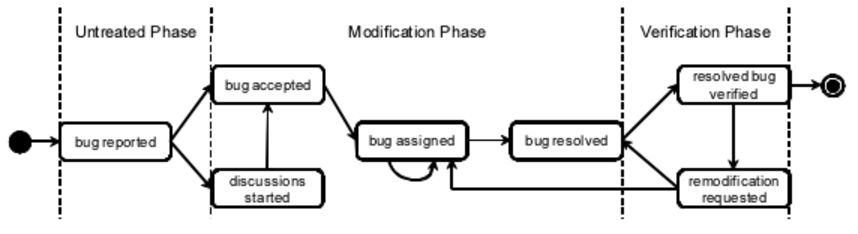
\includegraphics[width=0.8\linewidth]{./chapter-manutencao-software-visao-geral/img/diagrama-estado-rm-codigo-aberto.pdf}
	\caption{Um processo de modificação de uma RM utilizando uma FGRM\@. Extraído
	de~\cite{ihara2009analysis}}
\label{fig:diagrama-estado-rm-codigo-aberto}
\end{figure}

Os autores ponderam que apesar da maneira que uma RM é modificada pode alterar
em diferentes projetos, o diagrama é capaz de representar de maneira geral o
processo de transição de uma RM\@. O processo é composto de três fases
diferentes: \textit{não tratada (untreated), modificação (modification) e
    verificação (verification)}.

A fase \textit{não tratada} foca em um subprocesso em que as RMs são relatadas,
todavia, não foram aceitas ou atribuídas à algum membro da equipe. A fase de
\textit{modificação} é um subprocesso em que as RMs são efetivamente modificadas.
Nesta fase uma RM é aceita e posteriormente atribuída a algum desenvolvedor.
Caso o pedido da RM não possa ser atendido ela é \textit{rejeitada}.  A fase de
\textit{verificação} é o subprocesso em que membros com a responsabilidade de
garantia da qualidade verificam se as RMs modificadas foram efetivamente
solucionadas. Caso uma RM modificada por um desenvolver não seja verificada, ela
poderia não ser reconhecida como fechada (closed).

É possível relacionar o modelo descrito por Tripathy \&
Naik~\cite{tripathy2014software} e aquele proposto por Ihara e
outros~\cite{ihara2009analysis}. Em ambos é possível identificar fases em que uma
RM é relatada, analisada e verificada. Além disso, os modelos discriminam
situações em que o pedido descrito na RM não é capaz de ser realizado. Nesta
dissertação utilizamos de forma geral o modelo proposto por Ihara e outros. Nos
casos em que houver necessidade de um maior detalhamento a discussão tomará como
base o modelo de Tripathy \& Naik.

\subsubsection{Problemas e Desafios do Gerenciamento das RMs}
\label{ssub:problemas_relacionadas_rm}

A gestão das RMs é um desafio em projetos de software de diferentes tamanhos. A
literatura discute e apresenta alguns problemas sobre o gerenciamento das RMs. A
seguir discutimos os que do nosso ponto de vista são os mais relevantes.

\paragraph{Localização do Problema:}

A tarefa de encontrar a origem de uma falha de software é complexa e consome
muito tempo. O estudo de Lúcia e outros afirma que na faixa de 84 a 93\% de
problemas em software afetam entre 1 e 2 arquivos de
código-fonte~\cite{thung2012faults}. Apesar da pequena quantidade de arquivos
afetados, identificar em quais deles o problema reside (buggy files) é uma
tarefa árdua~\cite{Thung:2014:BIT:2635868.2661678}.

Neste contexto, pesquisadores vêm propondo abordagens baseadas em Recuperação da
Informação para localizar o arquivo que contém uma falha com base no texto do
relato de uma RM\@. Nesse tipo de abordagem existe a tentativa de encontrar um
elo entre o texto do relato e um conjunto de arquivos que podem estar
relacionados com a solução do problema~\cite{Wong:2014:BBF:2705615.2706096}.

\paragraph{Dificuldade na Visualização das Informações das RMs:}

Uma tomada de decisão deve ser subsidiada por informações corretas. Este fato
não é diferente na manutenção e desenvolvimento de software. Pouco se sabe sobre
o comportamento evolutivo, o tempo de vida, distribuição e estabilidade dos
problemas reportados nas FGRMs~\cite{hora2012bug}. Este problema é reforçado
pela forma como as FGRMs armazenam os dados das RMs. Em geral, essas ferramentas
exibem informações sobre as RMs de forma textual, o que não é apenas complicado
para navegar, mas também dificulta a compreensão dos problemas do
software~\cite{dal2014bug}. Por esta razão estudos estão sendo realizados de
modo a propor novas formas de visualização da informação contida nas
RMs~\cite{takama2013application,hora2012bug}.

\paragraph{Baixa Qualidade do Relato:}

Durante o processo de solução de uma RM a reprodução manual das falhas
reportadas é demorada e tediosa. Os mantenedores tentam reproduzir problemas
usando a informação contida nas RMs que muitas vezes está
incompleta~\cite{White:2015:GRR:2820282.2820291}. Em algumas situações, para
obter os dados que necessita, o desenvolvedor deve registrar um comentário para
que o responsável do relato inclua as informações necessárias~\cite{5070993}. A
melhoria da qualidade do relato pode implicar na redução do custo do processo de
garantia de qualidade bem como aumentar a confiabilidade do software com a
redução gradativa de falhas~\cite{Tu:2014:MQI:2677832.2677844}.

% \paragraph{Organização da Informação da RM:}

% Em alguns casos não é possível aumentar a qualidade da informação fornecida em
% um relato de uma RM antes que ela seja armazenada em seu respectivo repositório.
% Nestas situações uma abordagem adotada é organizar de uma maneira previamente
% definida as informações contidas em uma RM\@. Durante o processo de análise de
% uma RM, em especial para aquelas de caráter corretiva, existe a tendência dos
% desenvolvedores procurar por problemas semelhantes que foram resolvidos no
% passado.

\paragraph{Identificação de RMs Duplicadas:}

O processo de identificação de RMs Duplicadas consiste em avaliar se determinado
relato já foi realizado em outro momento. Quando uma RM é identificada como
duplicada ela deveria ser relacionada com a sua ``cópia''. Uma delas é definida
como RM Mestre e as demais RMs Filhas. Geralmente a Mestre é aquela que foi
primeiramente incluída no repositório de erros. Alguns estudos revelam que entre
10\% e 30\% das RMs podem ser classificadas como
duplicadas~\cite{anvik2005coping,cavalcanti2013bug,Runeson:2007:DDD:1248820.1248882}.
Por conta do grande número de RMs repetidas uma das soluções é o \textit{Agente
    de Triagem} analisá-las manualmente com objetivo de evitar que elas cheguem
aos desenvolvedores~\cite{anvik2005coping}. Em alguns casos esta solução não é
viável. O processo de identificação de RMs duplicadas requer: \textit{(i)} um
prévio conhecimento do conjunto de relatos existentes anteriormente no projeto;
\textit{(ii)} a busca manual em toda base de dados da
FGRM~\cite{banerjee2012automated,
    Lerch:2013:FDY:2495256.2495763,hindle2016contextual}. Ambas as estratégias
consomem tempo e não garantem que falsos positivos possam
ocorrer~\cite{kaushik2012comparative}. Os falsos positivos podem ainda acarretar
na desconsideração de problemas relevantes.

\paragraph{Atribuição (Triagem) de RM:}

O processo de atribuição de RMs, cuja principal atividade é conhecida como
\textit{triagem}, tem como objetivo encontrar o desenvolvedor mais capacitado
para manipular uma dada RM~\cite{cavalcanti2014challenges}. Existe a premissa de
que a escolha do desenvolvedor apropriado é crucial para obter em menor tempo a
so\-lu\-ção da RM~\cite{di2002approach}. Estudos também discutem que o processo
de atribuição deve considerar fatores tais como a carga de trabalho do
desenvolvedor e a prioridade da RM, dentre outros~\cite{aljarah2011selecting}.

\paragraph{Classificação da RM:}

Independentemente do tipo e tamanho de um projeto é importante determinar qual
tipo de manutenção deverá ser realizada para cada RM que é criada. Geralmente
este tipo de classificação é feita com base no texto que corresponde ao relato
da RM\@. A diversidade de categorias pode tornar a tarefa complexa pelo fato de
que em muitos casos não é fácil determinar os limites entre os
tipos~\cite{antoniol2008bug}. Por exemplo, a uma classificação incorreta de um
defeito que na verdade trata-se de uma melhoria pode acarretar em atrasos no
projeto~\cite{cavalcanti2014challenges}.

\paragraph{Estimativa de Esforço da RM:}

A gestão de custo e esforço de um projeto de manutenção passa pelo controle do
esforço necessário para solucionar suas RMs. Os estudos que discutem o esforço
para solução de uma RM utilizam três formas de
estimativa~\cite{cavalcanti2014challenges}: determinar o tempo para solucionar
novas RMs; definir os artefatos que são impactados por determinada RM (Análise
de Impacto); prever o número de novas RMs que poderão fazer parte do projeto. A
literatura sobre análise de impacto é bastante abrangente e pode envolver o
estudo de artefatos tais como documentos de requisitos e arquiteturas de
softwares, código fonte, registros (logs) de teste e assim por
diante~\cite{cavalcanti2014challenges}.  Apesar da inerente imprecisão deste
tipo de trabalho é importante salientar que estimar o esforço de uma RM é
importante para o gerenciamento do projeto porque ajuda alocar recurso de forma
mais eficiente~\cite{Bhattacharya:2011:BTP:1985441.1985472} e melhorar a
previsão do custo necessário para o lançamento de futuras versões do
sistema~\cite{Vijayakumar2014}.

\paragraph{Recomendação de RMs:}

Em alguns projetos, um membro experiente da equipe, geralmente ensina os
recém-chegados o que eles precisam fazer para solucionar uma RM\@. Todavia,
alocar um membro experiente de uma equipe por um longo tempo para ensinar um
novato nem sempre é possível ou desejável. A premissa é que o mentor poderia ser
mais útil fazendo tarefas mais importantes~\cite{malheiros2012source}. Por
exemplo, quando um novo desenvolvedor entra na equipe seria interessante que ele
resolvesse as RMs que tivessem um menor nível de dificuldade. Posteriormente,
quando o desenvolvedor ganhasse mais experiência, poderia aumentar o grau de
dificuldade das RMs que ele deve tratar. Este tipo de processo ocorre com certa
frequência em projetos de código aberto, em que a contribuição de desenvolvedores
externos ao projeto é fundamental. No entanto, encontrar um defeito apropriado
ao nível de conhecimento do desenvolvedor, bem como a correção apropriada para o
mesmo requer uma boa compreensão do projeto~\cite{Wang2011bug}.

Para facilitar a inclusão de novos desenvolvedores alguns estudos vêm se
dedicando ao desenvolvimento de sistemas de recomendação de
RMs~\cite{malheiros2012source, Wang2011bug}. Estes sistemas podem ajudar o
recém-chegado a solucionar uma RM mediante a apresentação do código fonte
potencialmente relevante que o ajudará na solução da RM do qual ficou
responsável~\cite{malheiros2012source}.

% O segundo tipo de abordagem pode ser vista como ambiente de exploração do
% repositório de RMs.  Esta funcionalidade permite que novos desenvolvedores
% pesquisem descrições das requisições que possam ser do seu interesse bem como
% dos artefatos relativos àquela RM (por exemplo, arquivos relacionados,
% desenvolvedores contribuintes, registros de comunicação)~\cite{Wang2011bug}.

\section{As Ferramentas de Gerenciamento de Requisições de Mudança (FGRM)}
\label{sec:ferramentas_de_gerenciamento_requisicoes_de_mudanca}

Dentro da disciplina de Gerenciamento da Configuração do Software a atividade de
controle de configuração é responsável por gerenciar mudanças ocorridas durante
o ciclo de vida de um produto de software~\cite{tripathy2014software}. Entre as
atividades deste processo estão determinar quais alterações serão feitas,
definir o papel responsável por autorizar certos tipos de mudanças e aprovar
desvios relativos aos requisitos iniciais do projeto~\cite{4425813}. De uma
forma mais ou menos estruturada tais ações ocorrem em diferentes tipos de
projeto de software, seja ele com características tradicionais (vide
Seção~\ref{subsec:manutenção_de_software_tradicional}) ou ainda naqueles que
utilizam os métodos propostos pelos agilistas.

Por conta do volume das RMs, e os diversos desafios relacionados com sua gestão,
é necessária a utilização de ferramentas com o objetivo de gerenciá-las. Esse
controle é geralmente realizado por Sistemas de Controle de Demandas (SCD)\@-\@
Issue Tracking Systems, que auxiliam os desenvolvedores na correção de forma
individual ou colaborativa de defeitos (bugs), no desenvolvimento de novas
funcionalidades, dentre outras tarefas relativas à manutenção de software. Não
existe na literatura uma nomenclatura padrão para este tipo de sistema. Em
alguns estudos é possível verificar nomes tais como Sistema de Controle de
Defeito\@-\@ Bug Tracking Systems, Sistema de Gerenciamento da Requisição\@-\@
Request Management System, Sistemas de Controle de Demandas (SCD)\@-\@ Issue
Tracking Systems. Todavia, de modo geral, o termo se refere às ferramentas
utilizadas pelas organizações para \textit{gerenciar as Requisições de Mudança}.
Estas ferramentas podem ainda ser utilizadas por gestores, analistas de
qualidade e usuários finais para atividades para gerenciamento de projetos,
comunicação, discussão e revisão de código. Neste trabalho utilizaremos o termo
\texttt{Ferramentas de Gerenciamento de Requisições de Mudança} (FGRM) ao nos
referir a este tipo de software.

As RMs são controladas por uma FGRM na forma de um fluxo de trabalho de modo a
identificar, descrever e controlar a sua situação. Em geral, os objetivos de um
projeto em adotar uma FGRM para gerenciar suas RMs são os
seguintes~\cite{tripathy2014software}:

\begin{itemize}
    \item Disponibilizar um espaço comum para a comunicação entre as partes
        interessadas.
	\item Identificar de forma única e controlar a situação de cada RM\@. Esta
		característica simplifica o processo de relatar uma RM e fornece um
		melhor controle sobre as mudanças.
    \item Manter uma base de dados sobre todas as mudanças no sistema
        desenvolvido ou mantido pelo projeto. Esta informação pode ser utilizada
        para monitoramento e métricas de medição.
\end{itemize}

No momento em que este trabalho estava sendo desenvolvido, estudos discutem o
fato de que as FGRMs não apenas ajudam as organizações a gerenciar, atribuir,
controlar, resolver e arquivar as RMs~\cite{Bertram:2010:CCB:1718918.1718972}.
Em alguns casos, este tipo de ferramenta se tornou o ponto focal para
comunicação e coordenação para diversas partes interessadas, dentro e além da
equipe de manutenção. As FGRMs servem como um repositório central para monitorar
o progresso das RMs, para solicitar informações adicionais da pessoa responsável
por redigir a requisição e o ponto de discussão para potenciais soluções de um
defeito (bug)~\cite{zimmermann2009improving}.

Em projetos de código aberto, as FGRMs são um importante espaço onde a equipe de
desenvolvimento interage com a comunidade. Como consequência é possível observar
o fenômeno da participação dos usuários no processo de solução da RM:\@ eles não
apenas submetem a RM, mas também participam da discussão de como resolvê-la.
Desta forma, o usuário final ajuda nas decisões sobre a direção futura do
produto de software~\cite{breu2010information}.

\subsection{Modelo Conceitual do Contexto das FGRMs}
\label{sub:espectro_funcionalidades_fgrm}

As FGRMs vêm sendo utilizadas por diversos projetos com características
próprias. Neste sentido, este tipo de software deveria oferecer diferentes
funcionalidades para que possa atender a diferentes demandas. Apesar da
variedade de ferramentas
disponíveis\footnote{\url{https://en.wikipedia.org/wiki/Comparison_of_issue-tracking_systems}}
é possível encontrar atributos comuns que permitem a compilação de um modelo
conceitual.

Nós construímos um modelo conceitual com base na literatura da área, em especial
nos trabalhos de~\cite{cavalcanti2014challenges, singh2011bug,
    kshirsagar2015issue}. Nós sintetizamos os dados através da identificação de
temas recorrentes da definição de FGRMs disponíveis naqueles artigos. Foram
encontrados quatro principais conceitos que estão retratados na
Figura~\ref{fig:diagrama-classe-conceitual-fgrm} como um diagrama baseado na
UML\@. Esta figura foi derivada dos estudos primários e consiste em uma
generalização de elementos utilizados com frequência nos estudos que nós
utilizamos. Os conceitos envolvidos no modelo estão descritos a seguir.

\begin{description}
	\item[Projeto:] Projeto de software para o qual a FGRM visa suportar.
		Ele é composto pelos atributos \textit{Componentes de Software},
		\textit{Artefatos} e \textit{Contexto de Desenvolvimento}.
		\begin{itemize}
			\item  \textit{Componente de Software} representa um ou mais módulo
				que fazem parte do sistema que a FGRM suporta.
			\item \textit{Artefatos} são os objetos utilizados ou produzidos no
				desenvolvimento do software tais como código fonte,
				documentação, casos de teste e etc.
			\item \textit{Contexto de Desenvolvimento} representa os atributos
				que interferem no processo de desenvolvimento e manutenção de
				software. Nele está contido o processo de desenvolvimento (por
				exemplo métodos ágeis, cascata, iterativo e etc), as ferramentas
				utilizadas (compiladores, ferramentas de debug e de build), dentre
                outros aspectos.
		\end{itemize}
	\item[Repositório de RM:] Trata-se da base de dados onde as RMs são
		armazenadas e gerenciadas. Cada item nesta base é uma RM com as
		características discutidas na Seção~\ref{sec:requisicao_de_mudanca}.
    \item[Repositório de Usuários] Representa a base de dados de usuários da
        FGRM\@. Nele são gerenciados os dados das pessoas envolvidas no projeto
        e de seus respectivos direitos de acesso às informações das RMs. Neste
        caso, esta base inclui tanto a equipe de manutenção quanto as demais
        partes interessadas.
	\item[Fluxo de Trabalho:] O \textit{Fluxo de Trabalho} representa o conjunto
		de regras que gerenciam o processo de solução das RMs\@. É a partir
		dele que são definidos os diferente \textit{estados} que uma RM pode
		assumir desde de quando ela é redigida até o momento em que se define
		que foi solucionada. Este processo é realizado pelas \textit{Pessoas}
		envolvidas no \textit{Projeto} através dos diferente \textit{Papéis}
		desempenhados e suas respectivas \textit{Atividades}. Uma discussão mais
		aprofundada sobre os papéis desempenhados na manutenção de software está
		disponível na
		Subseção~\ref{subsec:man_visao_geral_papeis_na_manutencao_de_software}.
		De maneira relacionada, os diferentes estados de um ciclo de vida de uma
		RM estão descritos na
		Subseção~\ref{sub:fluxo_de_trabalho_requisicao_mudanca}.
\end{description}

A partir da Figura~\ref{fig:diagrama-classe-conceitual-fgrm} é possível
verificar que um \textit{projeto} pode \textit{definir} o seu \textit{fluxo de
    trabalho}, como por exemplo resolvendo que uma RM só pode ser considerada
Fechada (Closed) \@-\@ vide Seção~\ref{sub:fluxo_de_trabalho_requisicao_mudanca}
\@-\@ caso ela tenha sido avaliada por um Analista de Qualidade (vide
Seção~\ref{subsec:man_visao_geral_papeis_na_manutencao_de_software}). A partir
deste fluxo as RMs podem ser \textit{atendidas} visando à sua solução o que é
feito por uma \textit{pessoa} devidamente registrada no \textit{repositório de
    pessoas} e com permissão para realizar a ação necessária.

\begin{figure}[htpb] \centering
	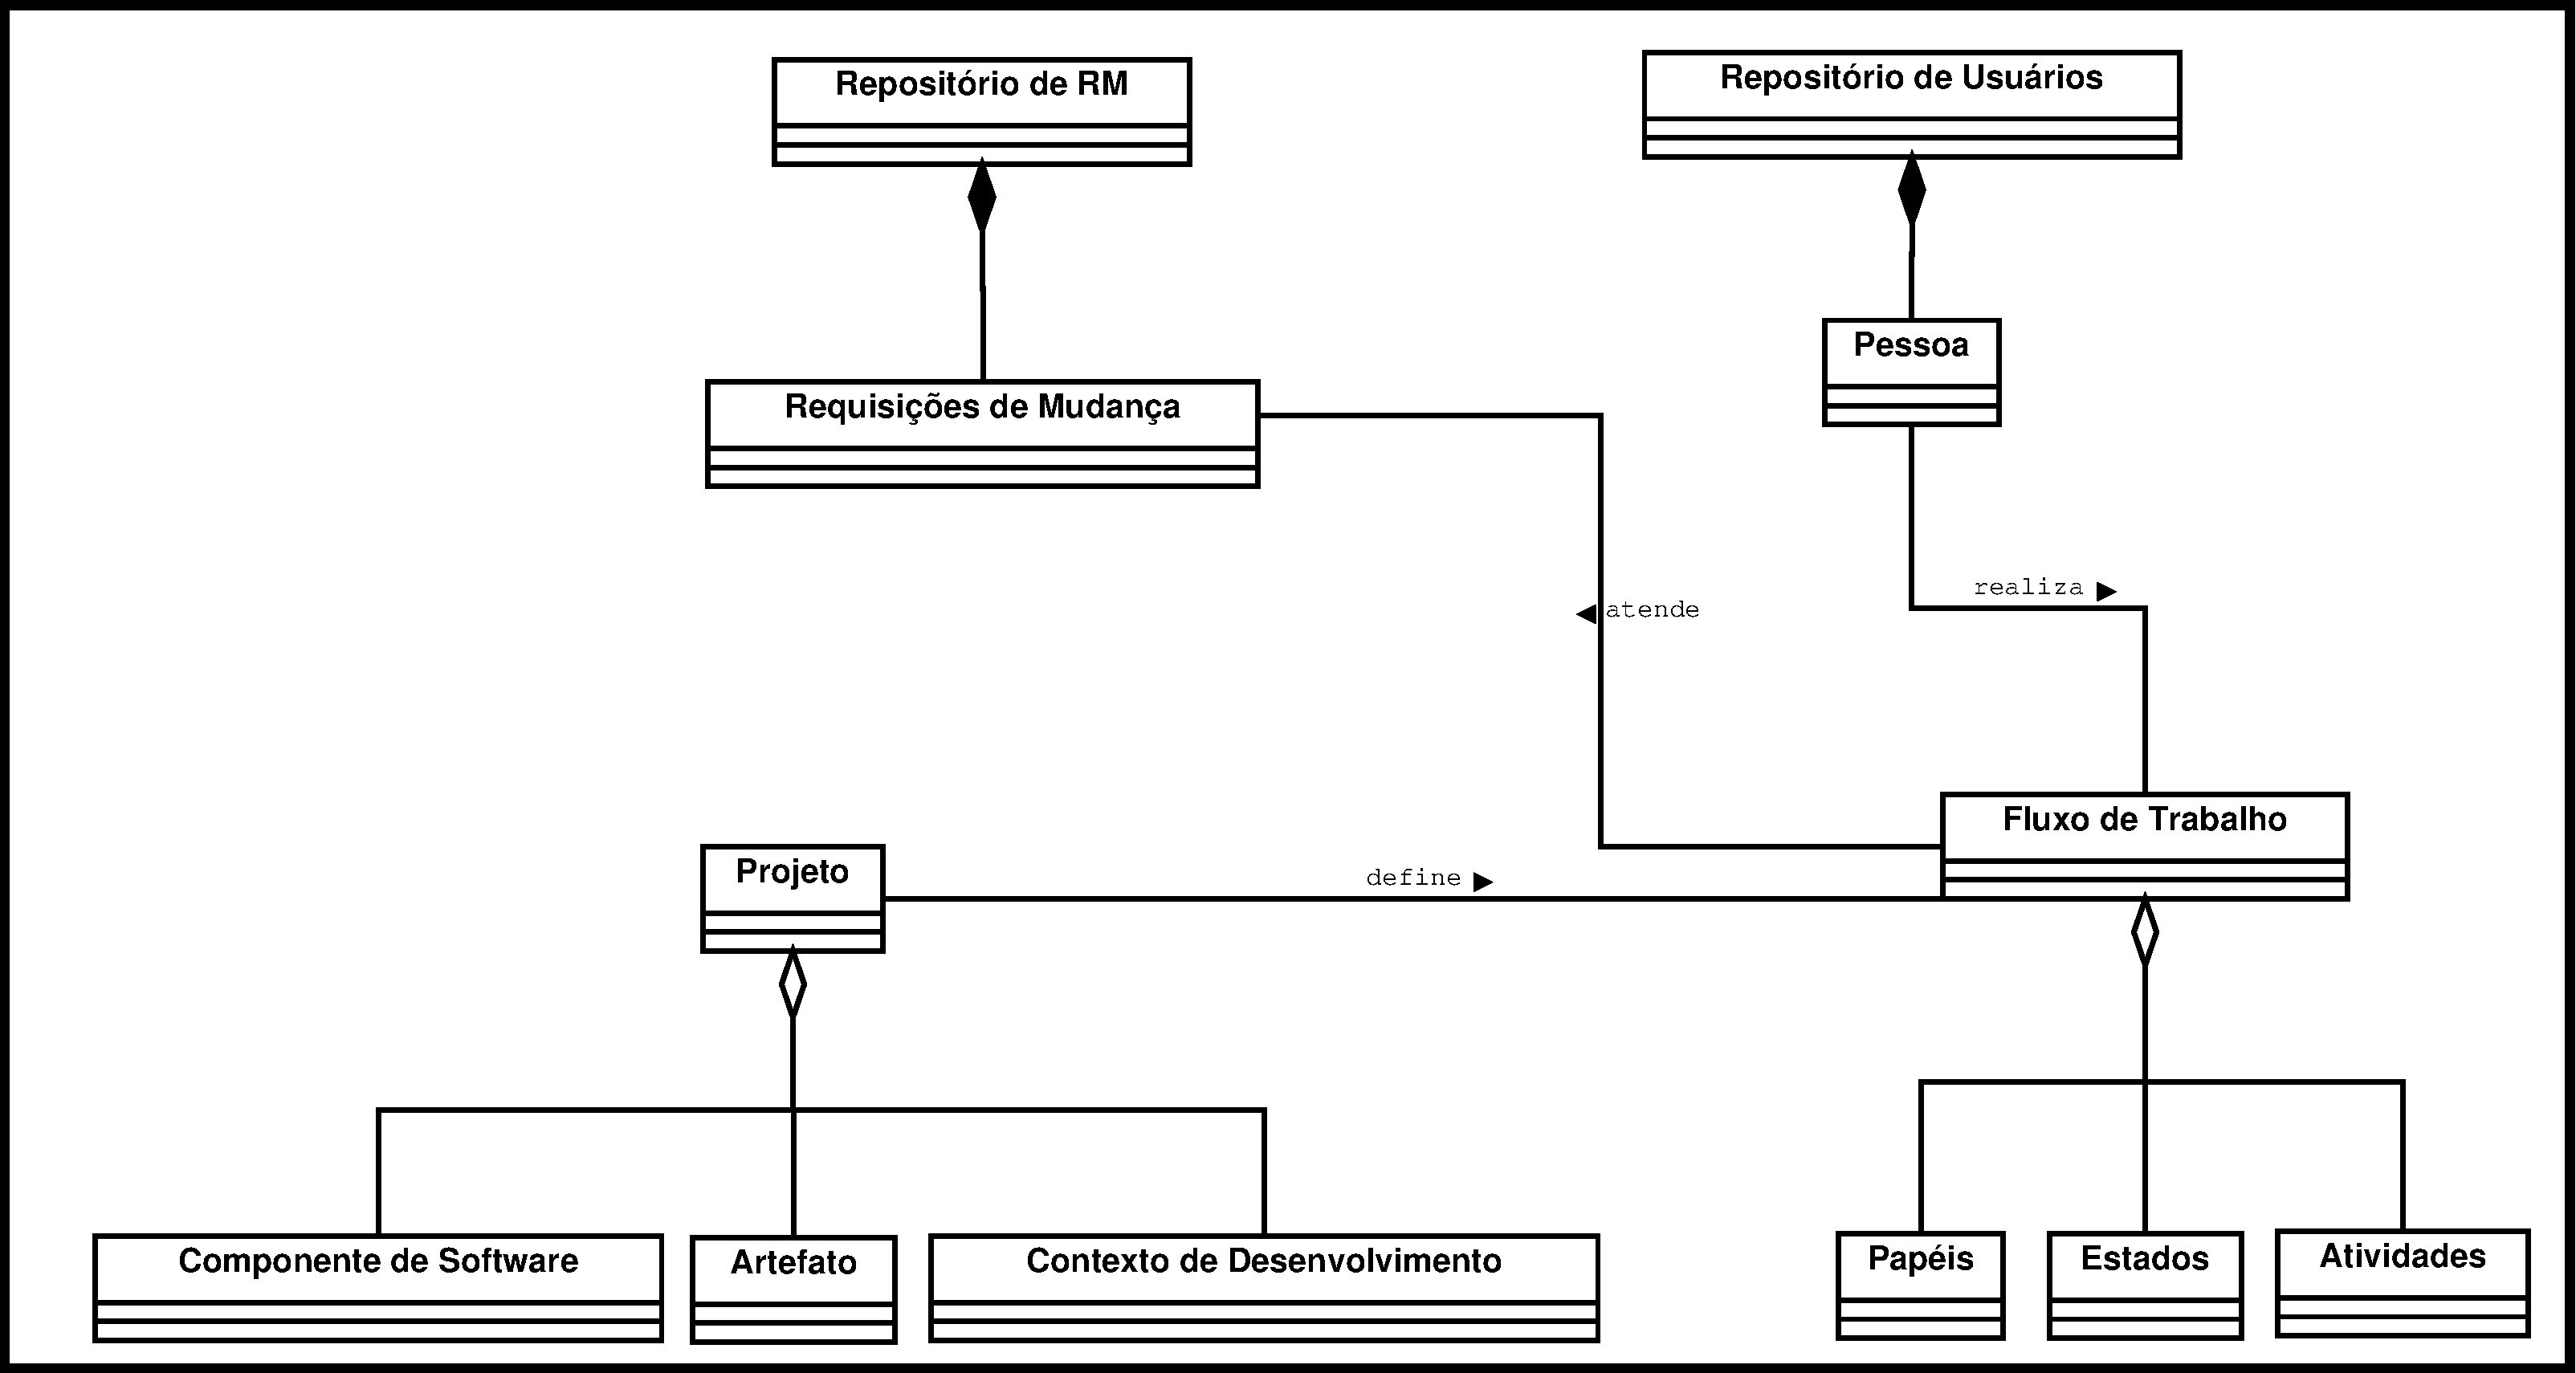
\includegraphics[width=1.15\linewidth]{./chapter-manutencao-software-visao-geral/img/diagrama-classe-conceitual-fgrm.pdf}
	\caption{Modelo conceitual do contexto de uma FGRM}
\label{fig:diagrama-classe-conceitual-fgrm}
\end{figure}

Conforme exposto, as FGRMs desempenham um papel que vai além de gerenciar as
Requisições de Mudança. Neste sentido, é importante estudar este tipo de
software em busca do conhecimento de como melhorá-los de modo a atender as
diversas necessidades dos seus usuários. Contudo, é importante avaliar as novas
funcionalidades propostas na li\-te\-ra\-tu\-ra. Uma possível forma de melhoria
é através do uso de extensões. Na próxima seção abordamos esta propriedade de
algumas FGRMs que permitem a inclusão e modificação de funcionalidades e
comportamentos segundo as necessidades do usuário.

\subsection{Extensões de Funcionalidades em FGRM}
\label{subsec:manutencao_visao_geral_extensoes_fgrm}

Em determinados domínios de aplicação é interessante desenvolver produtos de
software com uma arquitetura que permita o sistema se adaptar às mudanças em em
seu ambiente. Existe a possibilidade de incluir novas funcionalidades dentro das
já existentes no software, todavia, verificamos que sistemas que permitem
extensões apresentam os seguintes benefícios:

\begin{itemize}
    \item Extensibilidade: o software pode ser dinamicamente estendido mediante
        a inclusão de novos módulos de código que correspondem à novas
        características;
    \item Desenvolvimento em Paralelo: Quando os componentes não possuem certas
        dependências eles podem ser desenvolvidos em paralelo por times
        diferentes;
    \item Simplicidade: uma extensão tipicamente tem uma única funcionalidade,
        desta forma, permite um maior foco de quem desenvolve.
\end{itemize}

No escopo deste trabalho, uma extensão é um componente de software que adiciona
uma característica ou comportamento específico para um programa de
computador\footnote{\url{https://en.wikipedia.org/wiki/Plug-in\_(computing)}}.
Cabe-nos ressaltar que a nossa definição de extensão incluí aquelas que não
estão acopladas ao código de determinada FGRM\@. Por exemplo, a funcionalidade
de atribuição de uma RM está presente na maior parte das FGRMs, todavia, segundo
nossa definição, uma proposta de melhoria desta funcionalidade mediante uma
atribuição automatizada, por exemplo, será analisada como extensão mesmo que ela
não esteja efetivamente funcionando em alguma FGRM\@. Vamos a\-na\-li\-sar as
extensões de funcionalidade de forma independente se ela é oferecida baseada nos
mecanismos de extensão discutidos nesta seção.

Verificamos na literatura alguns estudos em que as soluções propostas já se
tornaram extensões de determinadas FGRM\@. Como pode ser observado no Mapeamento
Sistemático realizado no Capítulo~\ref{ch:mapeamento-sistematico}, a
implementação da proposta do estudo em extensão de ferramenta não é o padrão
observado. Os softwares que utilizam módulos de extensão têm aspectos de
desenvolvimento e de manutenção potencialmente distintos daqueles sem esta
característica. Este trabalho de mestrado faz uma contribuição na direção de uma
melhor compreensão deste contexto a partir da análise de aspectos específicos
das FGRMs.

% A extensão \textit{Buglocalizer}~\cite{Thung:2014:BIT:2635868.2661678} é uma
% extensão para o Bugzilla que possibilita a localização dos arquivos do código
% fonte que estão relacionados ao defeito relatado. A ferramenta extrai texto dos
% campos de sumário e descrição de um determinado erro reportado no Bugzilla. De
% maneira similar \textit{NextBug}~\cite{101186} também é uma extensão para o
% Bugzilla que recomenda novos bugs para um desenvolvedor baseado no defeito que
% ele esteja tratando atualmente. Em ambos os casos a extensão foi implementada
% utilizando técnicas de Recuperação da Informação.

\section{Um Estudo sobre as Funcionalidades das FGRMs}
\label{sec:caracterizacao_ferramentas}

\subsection{Visão Geral}
\label{subsec:caracterizacao_intro}

Quando uma empresa ou projeto de software de código aberto decide adotar uma
FGRM um desafio é encontrar aquela que melhor atenda suas necessidades.  Um
critério de seleção é o conjunto de funcionalidades oferecidas pelo software.
Outras variáveis podem envolver o custo e o suporte pós-venda da ferramenta. De
maneira relacionada, o pesquisador que estuda propostas de melhorias para as
FGRMs pode estar interessado em analisar o conjunto de funções que permita
caracterizar este tipo de software.

O número de FGRMs disponíveis quando esta dissertação foi escrita era bastante
elevado. Em uma inspeção inicial, verificamos a existência de mais de
\textit{50} ferramentas fornecidas comercialmente ou em código
aberto\footnote{\url{https://en.wikipedia.org/wiki/Comparison_of_issue-tracking_systems}}.
Apesar das diversas opções disponíveis, ao bem do nosso conhecimento,
desconhecemos estudos que avaliem sistematicamente as funcionalidades oferecidas
por este tipo de ferramenta. Entendemos que a partir de um conjunto
compartilhado de funções e comportamentos seja possível caracterizar as FGRMs,
ao mesmo tempo que possibilita avaliar a contribuição de novas funcionalidades
propostas na li\-te\-ra\-tu\-ra, conforme discutido no
Capítulo~\ref{ch:mapeamento-sistematico}. Com este objetivo realizamos um estudo
exploratório para coletar as funcionalidades presentes nas FGRMs. Em um estudo
exploratório a preocupação é analisar o objeto em sua configuração natural,
deixando que as descobertas surjam da própria
observação~\cite{wohlin2012experimentation}.

O estudo descrito nesta Seção consistiu na leitura da documentação disponível na
Internet de algumas FGRMs de modo a sistematizar as funcionalidades
o\-fe\-re\-ci\-das por cada ferramenta. As funções foram coletadas e organizadas
utilizando a técnica de Cartões de Classificação (Sorting Cards)~\cite{5070993,
    rugg2005sorting}. Devido ao alto volume de ferramentas disponíveis e ao
esforço necessário para analisar a documentação de todas elas, optamos por
realizar este estudo com um conjunto de 6 ferramentas que foram escolhidas com a
ajuda de profissionais envolvidos em manutenção de software. A opinião dos
profissionais foi coletada através de um levantamento por questionário (survey)
onde eles selecionavam as FGRMs que julgavam mais representativas dentre uma
lista previamente definida. A representatividade neste contexto não está no
número de projetos que utiliza determinada ferramenta, mas pelas caraterísticas
que o software possui e que o torna diferenciável dentro do seu domínio.

\subsection{Objetivo do Estudo}
\label{subsec:caracterizacao_objetivo_do_capitulo}

O objetivo deste estudo é apresentar e discutir as principais funcionalidades
das FGRMs que dão suporte ao desenvolvimento e manutenção de software. O ponto
de partida é o conjunto de sistemas escolhidos por meio de um levantamento
(survey). Acreditamos que o resultado permitirá uma melhor compreensão deste
tipo de software tomando como base o conjunto de funções que eles oferecem aos
seus usuários. Em um segundo momento também é possível propor novas
funcionalidades ou melhorias das existentes tendo em vista a possibilidade de
determinar o conjunto mínimo de comportamentos deste tipo de ferramenta.

\subsection{Metodologia}
\label{subsec:metodologia}

Para determinarmos o conjunto de funcionalidades das FGRMs realizamos um estudo
exploratório dividido nas três etapas listadas a seguir. O resultado obtido em
cada etapa foi utilizado para subsidiar as atividades da etapa subsequente. O
início de uma nova fase do trabalho era precedido de uma avaliação geral com o
objetivo de verificar possíveis inconsistências e avaliação das lições
aprendidas.

\begin{enumerate}[(i)]
	\item Seleção das Ferramentas
	\item Inspeção da Documentação
	\item Agrupamento das Funcionalidades
\end{enumerate}

\subsubsection{Seleção das Ferramentas}
\label{subsubsec:selecao-ferramentas}

A primeira etapa consistiu na definição das ferramentas que seriam utilizadas
no estudo. A partir de uma pesquisa na Internet obtivemos um conjunto inicial
de 50
ferramentas\footnote{\url{https://en.wikipedia.org/wiki/Comparison_of_issue-tracking_systems}}.
Devido ao esforço necessário e a dificuldade de realizar a análise em cada uma
optamos por escolher um subconjunto de sistemas que fossem mais
representativos, tomando como base a opinião de desenvolvedores de código
aberto e código proprietário, que tenham utilizado alguma FGRM\@. A
representatividade no escopo do levantamento corresponde a opinião do
profissional sobre notoriedade que a ferramenta possui dentro do seu domínio de
aplicação em comparação com as demais que lhe foram apresentadas ou outras do
qual o profissional tenha prévio conhecimento.

\subsubsection{Desenho do Levantamento por Questionário}
\label{ssub:metodologia_desenho_da_pesquisa_com_profissionais}

Para coletar a opinião dos profissionais utilizamos um formulário estruturado em
duas partes: a formação de base do participante (background) e a avaliação das
ferramentas. Na primeira, estávamos interessados em conhecer as características
do respondente. Esta informação é relevante para analisar de forma separada os
dois grupos de profissionais em que o questionário foi replicado. Na segunda,
apresentamos as ferramentas e solicitamos aos participantes que avaliassem a
relevância de cada uma delas através de uma escala do tipo
Likert~\cite{robbins2011plotting}. Foi disponibilizado aos participantes um
campo de texto livre em que era possível registrar outras FGRMs que ele entenda
relevante, mas que não estava na lista que lhe foi apresentada.

Antes da aplicação o questionário foi validado em um processo de três etapas. Na
primeira parte foi solicitada a avaliação por dois pesquisadores experientes da
área de Engenharia de Software. Após as alterações uma nova versão do formulário
foi enviada para dois profissionais que trabalham com manutenção de software. O
critério utilizado para seleção dos profissionais foi o tempo de experiência com
desenvolvimento e manutenção de software, que era em média de 10 anos. O
formulário foi modificado com as sugestões dos profissionais e isso finaliza a
segunda etapa de validação. A última etapa consistiu na realização de um piloto
com dez profissionais que trabalham em um setor manutenção de software de uma
empresa pública de informática. Trata-se de uma amostra de conveniência devida a
nossa facilidade de acesso a estes desenvolvedores. Os profissionais tiveram
que preencher o questionário, contudo, foram adicionadas questões em que era
possível inserir sugestões de melhoria. Como o público-alvo do questionário
poderia incluir desenvolvedores de diferentes nacionalidades foi criada uma
versão em língua inglesa.

No caso deste levantamento a população é o conjunto de profissionais que
trabalham com desenvolvimento e manutenção de software e que tenham uma razoável
experiência de uso com as FGRMs. A caracterização e estratificação desta
população não é simples. Neste sentido, visando minimizar possíveis
enviesamentos, replicamos o questionário em dois grupos:

\begin{description}
	\item[Grupo 01:] Profissionais que participam de fóruns e discussões sobre
		desenvolvimento e manutenção de software na rede social Stack Overflow.
	\item[Grupo 02:] Profissionais relacionados a grupos que contribuem em
		projetos de código aberto.
\end{description}

% A seleção dos potenciais participantes do levantamento foi utilizando os mesmo
% critérios que foram aplicados no estudo descrito na
% Seção~\ref{subsubsec:pesquisa_profissionais_plano_pesquisa}.

\subsubsection{Critérios de Seleção}
\label{ssub:metodologia_criterios_selecao}

Antes da seleção as FGRMs foram categorizados como \textit{''ferramentas''} e
\textit{''serviços da internet''}. Para incluir determinado software em um dos
grupos utilizamos a respectiva documentação do software. A primeira categoria
representa os softwares que são capazes de serem implantados na infraestrutura
do seu cliente e permite algum grau de personalização de pelo menos um dos
componentes, como por exemplo, o banco de dados utilizado. Na segunda estão os
software que oferecem o gerenciamento das RMs mediante uma arquitetura do tipo
Software como Serviço (Software as Service)~\cite{fox2013engineering}, onde
certos tipos de alterações no comportamento do software são mais restritas.
Acreditamos que ao escolher ferramentas dos dois tipos poderíamos cobrir grande
parte do domínio de aplicação das FGRMs. Optamos por escolher~\textit{03
    ferramentas} de cada categoria.

% Para seleção das ferramentas utilizados a formula apresentada na
% Equação~\ref{eq:escolha_ferramenta}. Atribuímos a métrica $r_i$ que representa a
% relevância de determinada ferramenta $f_i$.

O grupo final de FGRMs foi selecionado pela frequência com que cada grau de
relevância apareceu no formulário, conforme a Tabela~\ref{tab:graus_relevancia}.
Por exemplo, se uma ferramenta X teve a opção ``Muito relevante'' por três
profissionais ele recebe uma pontuação igual a 15. Caso uma ferramenta não
estivesse na lista, mas foi informada pelo participante de uma forma espontânea,
ela recebia uma pontuação igual a 5. Após o cálculo de pontuação de cada
ferramenta, ordenamos do maior para o menor valor e escolhemos as três melhores
posicionadas de cada categoria.

\begin{table}[htpb]
\centering
\begin{tabular}{@{}clc@{}}
\toprule
\textbf{\#} & \textbf{Grau de Relevância} & \textbf{Peso} \\ \midrule
1 & Não conheço a ferramenta & 1 \\
2 & Nada relevante & 2 \\
3 & Pouco relevante & 3 \\
4 & Pouco relevante & 4 \\
5 & Muito relevante & 5 \\ \bottomrule
\end{tabular}
\caption{Graus de Relevância}
\label{tab:graus_relevancia}
\end{table}

\subsubsection{Inspeção da Documentação}
\label{subsec:inspecao_doumentacao}

Nesta etapa do trabalho realizamos a leitura do material disponível na Internet
para cada uma das ferramentas selecionadas. Entre estes materiais utilizados
encontram-se manuais do usuário e do desenvolvedor e notas de lançamento. Para
cada uma das FGRMs optamos por estudar a última versão estável do software a fim
de analisarmos o que há de mais novo disponível aos usuários. A documentação de
algumas ferramentas, em especial aquelas que adotam uma arquitetura
cliente/servidor e necessitam de um certo grau de administração, dividem as
funcionalidades do software entre aquelas com foco no usuário final e
ad\-mi\-nis\-tra\-do\-res. Nestes casos, optamos por coletar as funcionalidades
cujo foco seja o usuário da FGRM, tendo em vista que administradores deste tipo
de software não serem o foco desta dissertação.

A Tabela~\ref{tab:fgrm-docs} apresenta as ferramentas analisadas e o elo de
ligação para os documentos utilizados neste estudo. Para aquelas ferramentas que
apresentam documentação em mais de um i\-di\-o\-ma optamos por utilizar aquela
escrita em inglês por entendermos que seja a mais atualizada.

\begin{table}[htpb]
\centering
\resizebox{\textwidth}{!}{%
\begin{tabular}{@{}ll@{}}
\toprule
\multicolumn{1}{c}{\textbf{Nome da Ferramenta}} & \multicolumn{1}{c}{\textbf{URL}} \\ \midrule
Bugzilla & \url{https://www.bugzilla.org/features/} \\
Github Issue Tracking System & \url{https://github.com/blog/411-github-issue-tracker} \\
Github Issue Tracking System & \url{https://github.com/features} \\
Github Issue Tracking System & \url{https://guides.github.com/features/issues/} \\
Gitlab Issue Tracking System & \url{http://docs.gitlab.com/ce/user/project/labels.html} \\
Gitlab Issue Tracking System & \url{https://about.gitlab.com/2016/08/22/announcing-the-gitlab-issue-board/} \\
Gitlab Issue Tracking System & \url{https://about.gitlab.com/solutions/issueboard/} \\
Gitlab Issue Tracking System & \url{https://docs.gitlab.com/ee/user/project/description\_templates.html} \\
Gitlab Issue Tracking System & \url{https://docs.gitlab.com/ee/user/project/issues/automatic\_issue\_closing.html} \\
Gitlab Issue Tracking System & \url{https://docs.gitlab.com/ee/workflow/issue\_weight.html} \\
Gitlab Issue Tracking System & \url{https://docs.gitlab.com/ee/workflow/milestones.html} \\
Gitlab Issue Tracking System & \url{https://docs.gitlab.com/ee/workflow/time\_tracking.html} \\
JIRA & \url{https://br.atlassian.com/software/jira/features} \\
MantisBT & \url{https://www.mantisbt.org/wiki/doku.php/mantisbt:features} \\
Redmine & \url{http://www.redmine.org/projects/redmine/wiki/Features} \\ \bottomrule
\end{tabular}%
}
\caption{Documentações utilizadas no processo de coleta de dados.}
\label{tab:fgrm-docs}
\end{table}

Os dados obtidos da leitura dos materiais disponíveis para cada ferramenta foram
sistematizados por meio de técnica denominada \textit{Cartões de
    Classificação~-~Sorting Cards}. Trata-se de uma processo de elicitação de
conhecimento de baixo custo e com foco no usuário. Ela é utilizada na área de
arquitetura da informação para criar modelos mentais e derivar uma classificação
a partir dos dados utilizados~\cite{just2008towards}. A técnica envolve a
categorização de um conjunto de cartões em grupos distintos de acordo com algum
critério previamente definido~\cite{mcgee2009software}. O estudo de Maiden e
outros~\cite{maiden1996acre} sugere que os Cartões de Classificação seja uma das
mais úteis para aquisição de conhecimento de dados, em contraste ao conhecimento
de comportamento ou de processo.

Existem três principais fases dentro do processo de Classificação dos Cartões:
($i$) preparação, no qual participantes ou o conteúdo dos cartões são
selecionados; ($ii$) execução, em que os cartões são organizados em grupo
significativos com um título que o descreve; e por fim, ($iii$) análise, no qual
os cartões são sistematizados para formar hierarquias mais abstratas e que são
usadas para deduzir resultados. No processo tradicional de Cartões Ordenados
cada declaração realizada por um participante resulta na criação de exatamente
um único cartão~\cite{just2008towards}. Contudo, no nosso caso, foi realizada a
divisão da documentação da ferramenta por cada funcionalidade encontrada. Neste
sentido, cada funcionalidade obtida mediante a inspeção da documentação foi
mapeada em um único cartão.

Os cartões foram organizados de modo que continham o nome e a versão da
ferramenta analisada; a URL da documentação utilizada; o nome da funcionalidade
coletada, que consiste de uma descrição breve conforme existente na
documentação; descrição detalhada da funcionalidade, cujo objetivo é facilitar o
processo de agrupamento que será descrito na próxima seção. Nas
Figura~\ref{fig:documentacao_bugzilla} e~\ref{fig:exemplo_cartao_ordenado} é
possível visualizar, respectivamente, a documentação de uma funcionalidade da
ferramenta Bugzilla e o cartão produzido.

\begin{figure}[htpb]
	\centering
	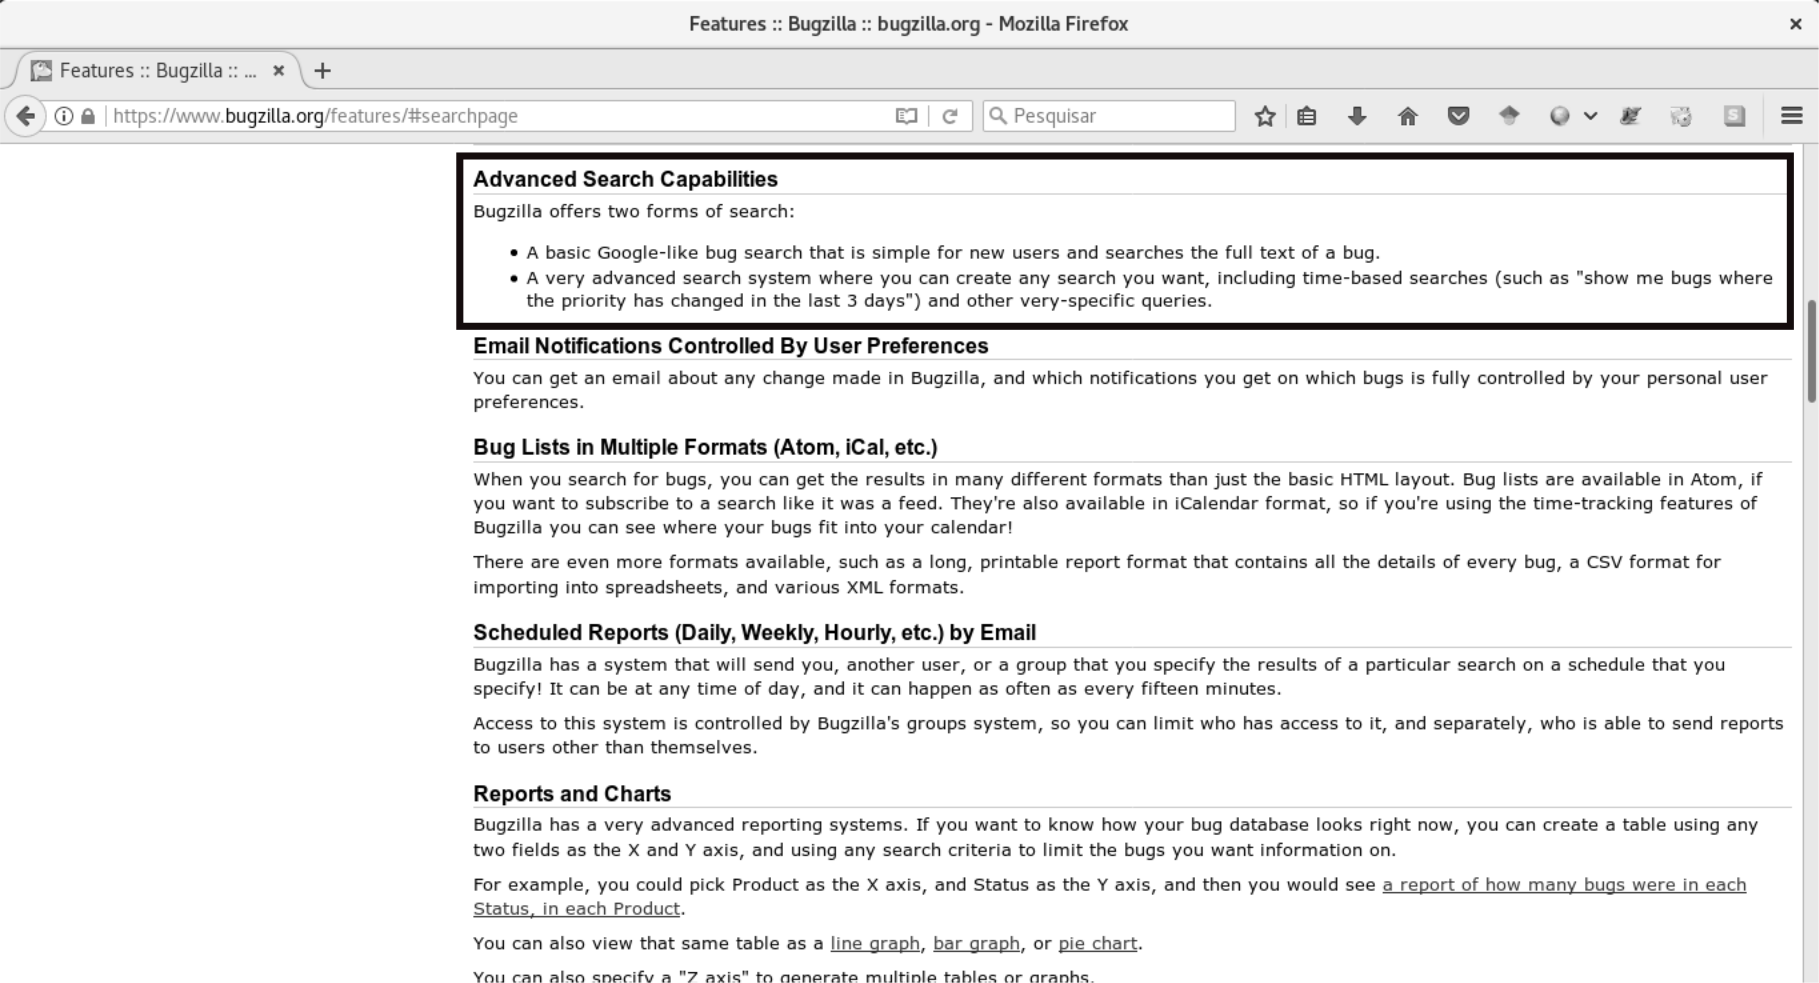
\includegraphics[width=0.9\linewidth]{./chapter-estudo-funcionalidades-fgrm/img/documentacao_bugzilla.png}
	\caption{Exemplo de documentação de uma funcionalidade da FGRM Bugzilla}
\label{fig:documentacao_bugzilla}
\end{figure}

\begin{figure}[htpb]
	\centering
	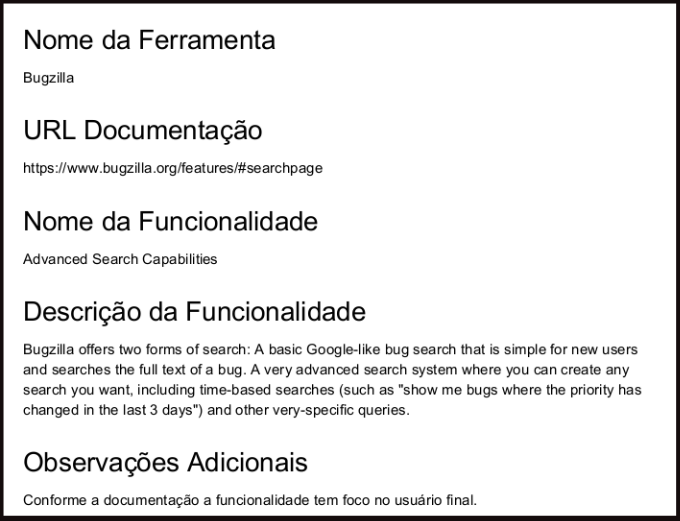
\includegraphics[width=0.5\linewidth]{./chapter-estudo-funcionalidades-fgrm/img/exemplo_cartao_ordenado.png}
	\caption{Exemplo de um cartão ordenado para uma funcionalidade da FGRM
		Bugzilla}
\label{fig:exemplo_cartao_ordenado}
\end{figure}

\subsubsection{Agrupamento das Funcionalidades}
\label{subsec:agrupamento_fucionalidades}

Esta etapa tem por objetivo agrupar as funcionalidades que aparecem com
nomenclatura distintas em diferentes ferramentas, mas que apresentam o mesmo
significado. Cabe ressaltar que o agrupamento de algumas funcionalidades pode
depender de uma análise subjetiva do responsável pela atividade. Neste sentido,
a fim de evitar algum tipo de viés, o agrupamento foi realizado em duas etapas:

\begin{description}
	\item[Análise Individual] Nesta etapa o autor e um outro especialista
		realizam de forma separada os agrupamentos.
	\item[Anaĺise Compartilhada] Em um segundo momento tanto o autor quanto o
		es\-pe\-ci\-a\-lis\-ta discutem as possíveis divergências até que um
		consenso seja obtido.
\end{description}

Após o processo de agrupamento foi possível realizar a categorização das
funcionalidades das ferramentas. Os resultados do processo de agrupamento são
apresentados e discutidos nas próximas seções.

\subsection{Resultados}
\label{sec:resultados}

Nesta seção iniciamos apresentando o perfil dos participantes e em seguida
exibimos as categorias resultantes do processo de ordenamento dos cartões.

\subsubsection{Perfil dos Participantes}
\label{ssub:perfil_participantes}

Ao final do levantamento realizado com profissionais obtivemos um total de
\textit{52} respostas. Os profissionais que participaram são em sua maioria
desenvolvedores conforme pode ser verificado na
Figura~\ref{fig:grafico_escolha_ferramentas_funcao_participantes}. O grupo de
respondentes também incluem Engenheiros de Software, Gerentes de Equipe e
Arquitetos de Software que, junto com os Desenvolvedores, representam mais de
80\% do total. Com relação a experiência verificamos que a maior parte possui
entre 3 e 10 anos (60\%). Na segunda posição temos os participantes com 10~-~20
anos de experiência (17\%). Com relação ao tamanho da equipe de que os
participantes fazem parte, verificamos uma prevalência de equipes de médio (mais
do que 10 membro) e pequenas (2 a 5 membros) porte. Por sua vez, estas equipes
estão predominantemente em empresas privadas de software, que representou 37
participantes. Com relação ao local de trabalho verificamos ainda que o segundo
posto em número de par\-ti\-ci\-pan\-tes ficou para empresas que pertencem ao
setor governamental, do qual tivemos 11 participantes. O restante é composto por
um profissional que se dedica a projetos de software livre e um estudante.

\begin{figure}[htpb]
	\centering
	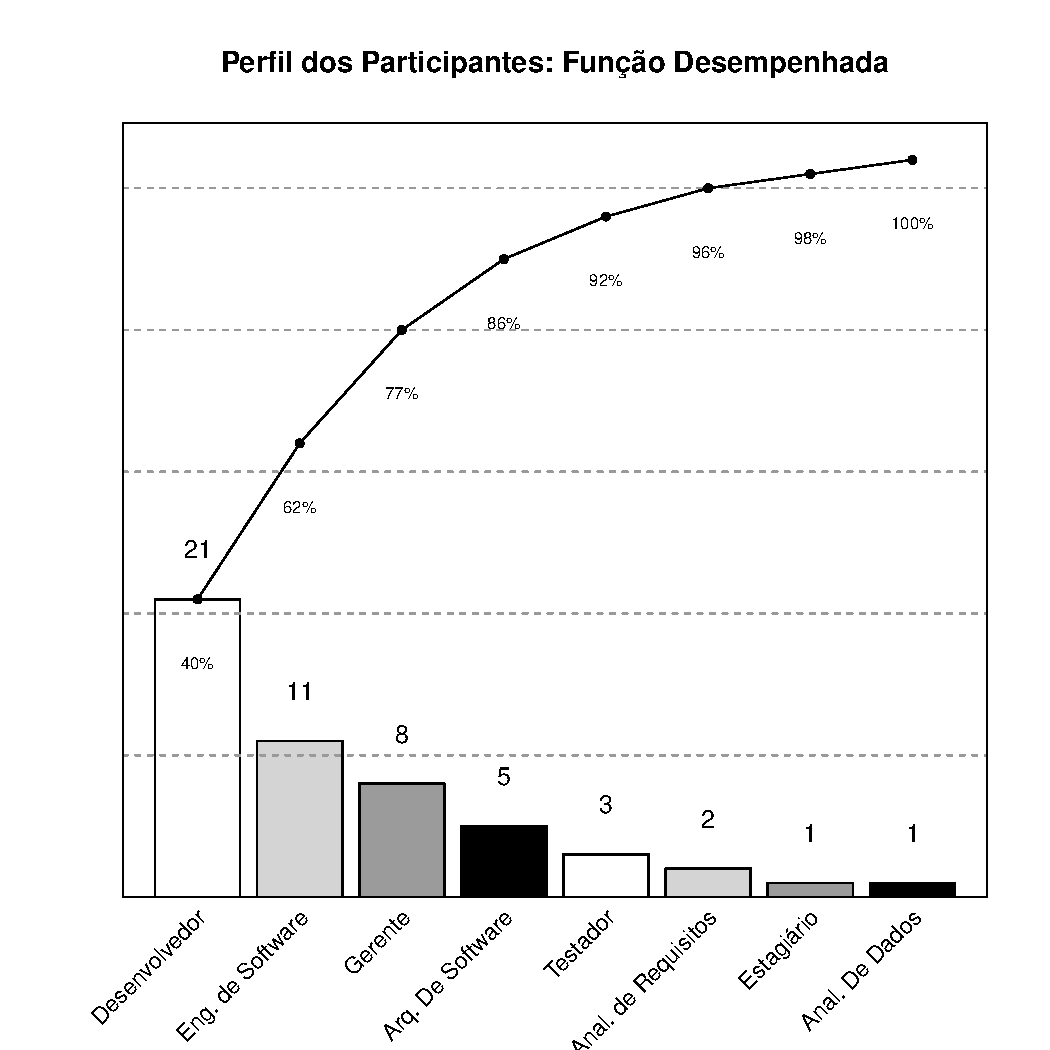
\includegraphics[width=0.5\linewidth]{./chapter-estudo-funcionalidades-fgrm/img/grafico_escolha_ferramentas_funcao_participantes.pdf}
	\caption{Funções desempenhadas pelos participantes}
\label{fig:grafico_escolha_ferramentas_funcao_participantes}
\end{figure}

Em geral, podemos caracterizar o participante típico como um desenvolvedor entre
três e dez anos de experiência trabalhando em uma empresa privada de
desenvolvimento de software com uma equipe de aproximadamente dez membros. Este
perfil profissional tem o conhecimento necessário para nos ajudar no processo de
escolha das ferramentas.

\subsubsection{Ferramentas Escolhidas}
\label{subsec:resultados_ferramentas_escolhidas}

O processo de seleção resultou nas ferramentas apresentas na
Tabela~\ref{tab:ferramenta_utilizadas_estudo}. Conforme pode ser observado foi
escolhido três softwares de cada tipo (ferramenta e serviço da Internet). É
importante perceber que as FGRMs \textit{Github e Gitlab} não estavam na lista
inicial, contudo, apareceram no resultado final. Isso decorre de atribuirmos o
maior peso para aquelas ferramentas que foram citadas pelos participantes de
maneira espontânea.

\begin{table}[htpb]
\centering
\resizebox{\textwidth}{!}{%
\begin{tabular}{lccl}
\toprule
\multicolumn{1}{c}{\textbf{Ferramenta}} & \textbf{\textbf{Classificação}} &
\textbf{Versão} & \multicolumn{1}{c}{URL} \\
\bottomrule
Bugzilla & Ferramenta & 5.0.3 & https://www.bugzilla.org \\
Mantis Bug Tracker & Ferramenta & 1.3.2 & https://www.mantisbt.org \\
Redmine & Ferramenta & 3.3.1 & http://www.redmine.org/ \\
JIRA Software & Serviço & 7.2.4 & https://br.atlassian.com/software/jira \\
Github Issue System & Serviço & \@-\@ & https://github.com/ \\
Gitlab Issue Tracking System & Serviço & \@-\@ & https://gitlab.com/ \\ 
\bottomrule
\end{tabular}%
}
\caption{Ferramentas utilizados no estudo}
\label{tab:ferramenta_utilizadas_estudo}
\end{table}


\subsubsection{Espectro de Funcionalidades das FGRMs}
\label{subsec:categorizacao_ferramentas}

Após a inspeção da documentação e validação dos dados obtivemos um total de 123
cartões. Nós sistematizamos os cartões manualmente tendo em vista que não
existem ferramentas ou métodos capazes de automatizar o processo de construção
deste tipo de hierarquia. Como o nosso objetivo é derivar tópicos a partir de um
conjunto inicial de cartões, optamos por realizar um \textit{ordenamento
    aberto}. Neste tipo de abordagem, os grupos são estabelecidos durante o
processo de classificação dos cartões em oposição a outra forma de utilização da
técnica em que a sistematização dos cartões ocorre com base em grupos
pré-determinados. Ao final do processo compilamos os tópicos de modo a construir
um espectro de funcionalidades para as FGRMs exibido na
Figura~\ref{fig:diagrama-espectro-funcionalidades-fgrm}.

\begin{figure}[htpb]
	\centering
	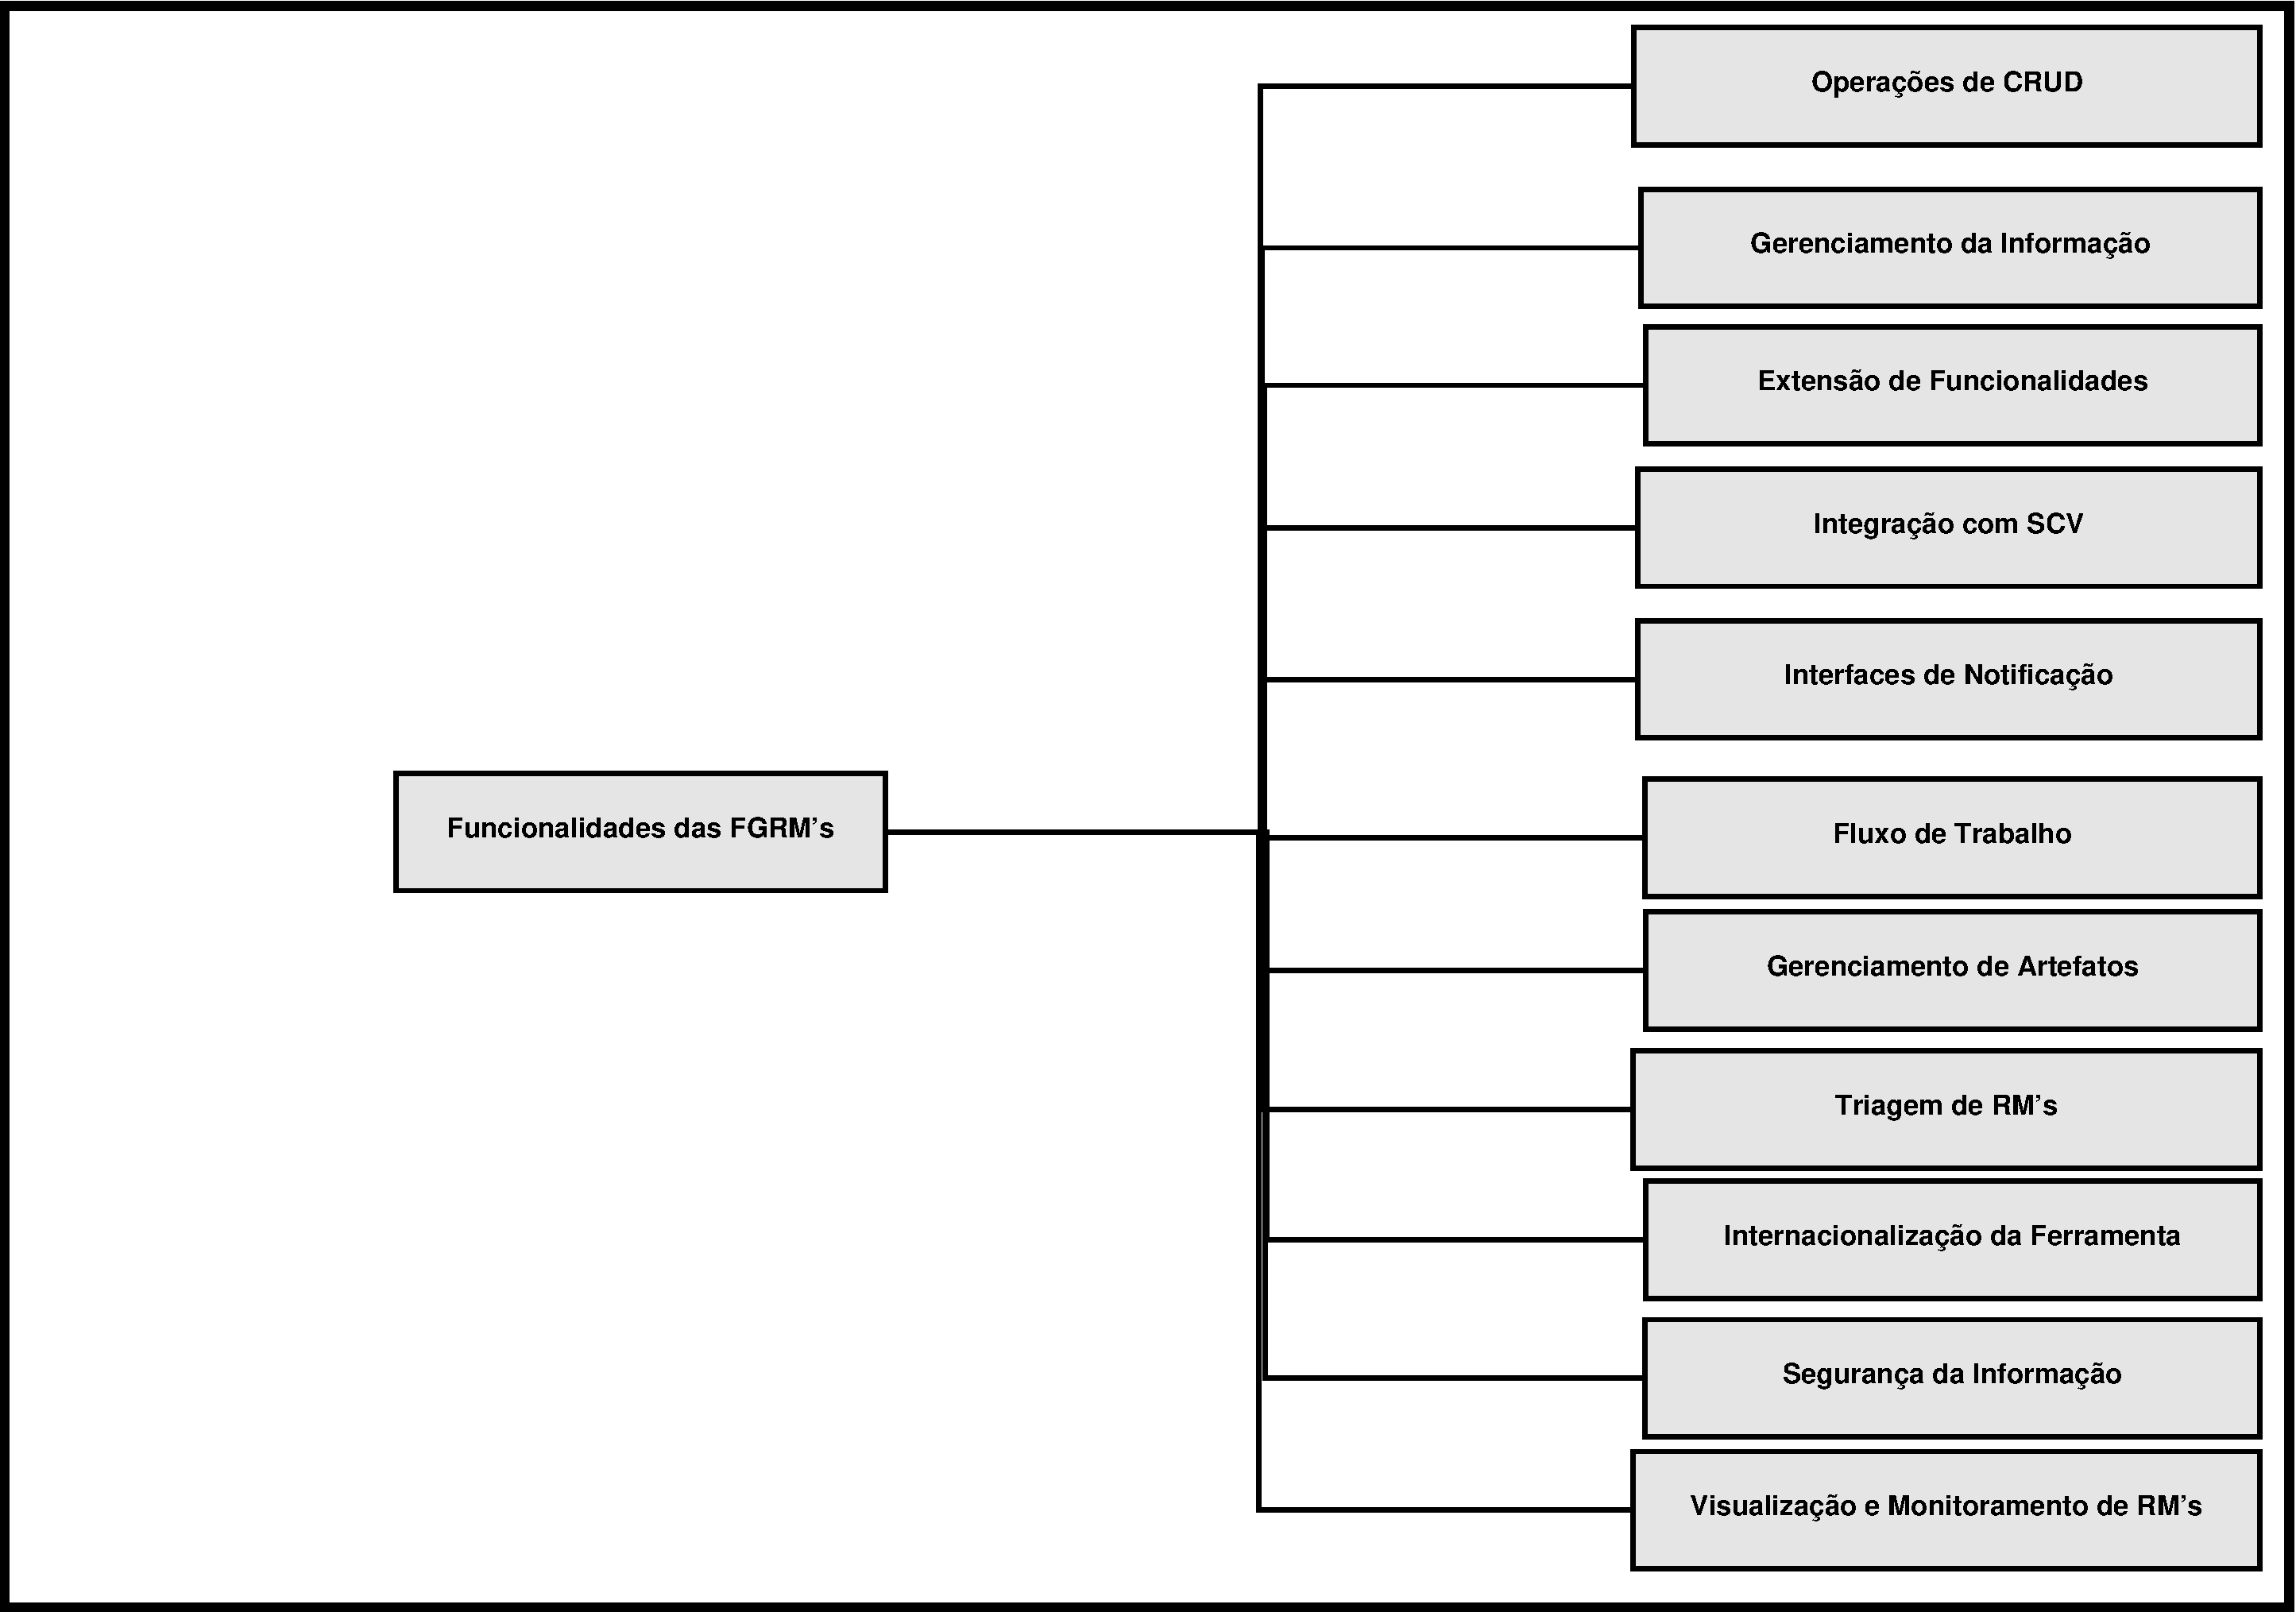
\includegraphics[width=1.15\linewidth]{./chapter-estudo-funcionalidades-fgrm/img/diagrama-espectro-funcionalidades-fgrm.pdf}
	\caption{Modelo de funcionalidades básicas das FGRMs}
\label{fig:diagrama-espectro-funcionalidades-fgrm}
\end{figure}

A figura foi construída com base nas categorias de funcionalidades exibidas na
Tabela~\ref{tab:freq_categorias_cartoes} em que é possível verificar a
frequência que cada uma das categorias apareceu no conjunto de cartões
coletados.

\begin{table}[htpb]
\centering
\resizebox{.7\textwidth}{!}{%
\begin{tabular}{lc}
\toprule
\multicolumn{1}{c}{\textbf{Categoria de Funcionalidades}} & \textbf{\textbf{Frequência}} \\ 
\bottomrule
Operações de CRUD & 24 \\
Visualização e Monitoramento de RMs & 22 \\
Segurança da Informação & 17 \\
Fluxo de Trabalho & 15 \\
Interfaces de Notificação & 13 \\
Extensão de Funcionalidades & 8 \\
Triagem de RMs & 6 \\
Gerenciamento de Artefatos & 6 \\
Integração com Sistemas de Controle de Versão & 4 \\
Gerenciamento da Informação & 4 \\
Internacionalização da Ferramenta & 3 \\
Auditoria & 1 \\
\bottomrule
\end{tabular}%
}
\caption{Frequência de cada categoria de funcionalidade no conjunto de cartões
	obtidos.}
\label{tab:freq_categorias_cartoes}
\end{table}

O gerenciamento das RMs formam as funcionalidades centrais de uma FGRM\@. De uma
maneira geral, uma das primeiras responsabilidades de uma FGRM é gerir a
\textit{criação, consulta, atualização e destruição} de uma RM\@. Estas funções
podem ser agrupadas em um termo único denominado \textit{Operações de CRUD}
(acrônimo de Create, Read, Update e Delete na língua Inglesa). As principais
categorias de funcionalidades que foram encontradas estão descritas a seguir.

\paragraph{Operações de CRUD:}
\label{par:operações_de_crud}

Nesta categoria estão as funcionalidades que dão suporte à criação,	consulta,
atualização e destruição das RMs. Com relação à criação verificamos que algumas
FGRMs permitem a definição de \textit{campos personalizáveis} para o
preenchimento da RM\@. A ferramenta Bugzilla suporta a atuação sobre um campo
personalizado de modo à capturar e pesquisar dados que são exclusivo do projeto
ao qual pertence. Estes campos podem ainda ser exibidos com base no valor de
outro, para usá-los apenas quando for de interesse.

Esta categoria também agrupa as funcionalidades relacionadas a busca de RMs e a
localização de duplicados. Durante o processo de criação de uma RM, uma das
ferramentas possui a funcionalidade para detecção automatizada de duplicados.
Para criar RMs algumas ferramentas possibilitam diferentes \textit{interfaces de
    entrada} de modo que ela pode ser criada através do envio de e-mail,
utilizando dispositivos móveis ou mediante formulários próprios criados em
qualquer site da web.

Verificamos ainda que algumas FGRMs permitem que o relato da RM seja realizado
em linguagem de marcação como o
Markdown\footnote{\url{https://en.wikipedia.org/wiki/Markdown}}, que permite,
dentre outras opções, a inclusão de código fonte com a sintaxe realçada. Isso
possibilita visualizar de forma mais clara partes do código que podem ser
incluídas. Neste mesmo tópico encontramos funcionalidades para recuperação das
RMs utilizando o texto contido no atributo que corresponde ao relato mediante
filtros personalizáveis ou por meio de uma Linguagem de Domínio Específico
(Domain-Specific Language \@-\@ DSL em inglês) baseada em SQL\@.

\paragraph{Gerenciamento da Informação}
\label{par:gerenciamento_da_informação}

Dentro de um projeto de desenvolvimento ou manutenção de software gerenciar uma
RM por vez não é muito eficiente. Neste sentido, é necessário que as FGRMs
permitam o gerenciamento em massa da informação armazenada. Este tópico
contempla as funcionalidades que se dedicam ao armazenamento e consistência das
informações contidas na FGRM\@. As ferramentas possuem funcionalidades para
\textit{suportar múltiplas bases de dados}, como suporte aos diferentes Sistemas
de Gerenciamento de Banco de Dados disponíveis no mercado. Além disso, a
ferramenta Bugzilla oferece funcionalidade para validação de consistências dos
dados armazenados.

As FGRMs devem fornecer recursos através dos quais outras ferramentas possam
interagir e manipular a informação que elas armazenam. Nesta dimensão estão as
funcionalidades que permitem manipulação externa dos dados contidos nas RMs ou
mesmo o desenvolvimento de novas funções ou comportamentos da FGRM mediante o
uso de
APIs\footnote{\url{https://en.wikipedia.org/wiki/Application_programming_interface}}
e extensões.

\paragraph{Extensão de Funcionalidades}
\label{par:extensão_de_funcionalidades}

As funcionalidades que compõem este grupo têm por objetivo estender o conjunto
de comportamentos oferecidos através de uma arquitetura de plugins ou mediante o
suporte de APIs. Algumas ferramentas como o Github permitem realizar as
atividades de gestão de uma RM mediante a utilização de uma API própria. No caso
do Bugzilla e do Mantis é permitido o acesso à informação das RMs através de
Webservices.

\paragraph{Integração com Sistemas de Controle de Versão}
\label{par:integração_com_sistemas_de_controle_de_versão}

As FGRMs podem acessar os repositórios de código de fonte, gerenciados mediante
um Sistema de Controle de Versão (SCV), permitindo que o usuário navegue pelo
seu conteúdo, visualize e procure o conjunto de alterações realizadas. As
ferramentas também possibilitam acesso à diferentes tipos de SCV, tais como Git,
SVN, Mercurial e etc.

\paragraph{Interfaces de Notificação}
\label{par:interfaces_de_notificação}

Neste tópico estão as funcionalidades oferecidas pelas FGRMs para notificar as
diversas partes interessadas envolvidas em determinado projeto de software. As
FGRMs podem notificar através de e-mail, RSS, Twitter e chats.

\paragraph{Fluxo de trabalho}
\label{par:fluxo_de_trabalho}

Nesta categoria estão as funcionalidades que dão suporte ao processo de trabalho
adotado no desenvolvimento e manutenção de software. Nela estão incluídos
dispositivos para gerenciamento de tarefas e suporte à múltiplos projetos.
Também é possível personalizar o fluxo de trabalho adotado. Esta customização é
realizada através da definição de \textit{situações} próprias que se adéquem às
necessidades do projeto.

\paragraph{Gerenciamento de Artefatos}
\label{par:gerenciamento_de_artefatos}

O processo de manutenção de software pode consumir ou gerar diversos artefatos,
tais como documentos de requisitos e arquiteturais dos software, código fonte,
registros (logs) de teste e assim por diante~\cite{cavalcanti2013bug}. Em alguns
contextos, devido ao volume de artefato gerados, é importante que a FGRM dê
suporte para armazenamento e recuperação deste ativos do processo de software.
As FGRMs possuem funcionalidades que interagem diretamente com a documentação
de software, geralmente no formato de Wikis. Além disso, algumas ferramentas
permitem uma melhor visualização de anexos incluídos na RM, como por
exemplo arquivos no formato CSV\@.

\paragraph{Triagem de RMs}
\label{par:triagem_de_rm_s}

Este tópico descreve as funcionalidades relacionadas com o processo de triagem
de RMs. As FGRMs dão suporte a esta atividade principalmente através da
categorização das RMs. Todas as ferramentas analisadas permitem algum tipo de
classificação através do uso de etiquetas.

\paragraph{Internacionalização da Ferramenta}
\label{par:internacionalização_da_ferramenta}

Neste tópico estão as características das FGRMs que ajudam no desenvolvimento
e/ou adaptação de um produto, em geral softwares de computadores, para uma
língua e cultura de um país. As FGRMs possuem tradução para diversos idiomas e
também possuem funcionalidades que permitem à colaboradores criarem novas
traduções.

\paragraph{Segurança da Informação}
\label{par:segurança_da_informação}

Neste grupo estão as funcionalidades de uma FGRM que estão diretamente
relacionadas com proteção de um conjunto de informações, no sentido de preservar
o valor que possuem para um indivíduo ou uma organização. Assim as ferramentas
oferecem funcionalidades para suporte à confidencialidade, integridade e
autenticidade da informação armazenada.

\paragraph{Visualização e Monitoramento de RMs}
\label{par:visualização_de_rm_s}

Em diversos contextos, devido ao volume das RMs, é importante que as partes
interessadas na manutenção de software, possam visualizar e monitorar a situação
das requisições que serão analisadas em determinado período. Neste contexto, as
FGRMs oferecem funcionalidades para visualizar a informação das RMs mediante
quadro como aqueles utilizados nas metodologias Kanban ou SCRUM\@. Existem
funcionalidades que permitem ao usuário visualizar um conjunto específico de
RMs. Neste mesma categoria estão as funcionalidades para geração de relatório
que ajudam aos gerentes do projeto na tomada de decisão.

\subsection{Discussão}
\label{sec:discussao}

Para algumas funcionalidades não há uma separação clara em qual categoria ela
pode ser encaixada, como por exemplo a possibilidade que algumas FGRMs fornecem
de personalizar os campos que compõem uma RM\@. Esta função está relacionada com
a criação da RM (Operação de CRUD), contudo, também faz parte da definição de
processo de trabalho próprio de um projeto, o que poderia categorizá-la como
Fluxo de Trabalho. Esta mesma situação ocorre com as funcionalidades de deleção
de uma RM que foram classificadas como \textit{Operações de CRUD}, mas que tem
relação com a categoria de \textit{Segurança da Informação} já que para realizar
tal ação o usuário deve ser identificado (login realizado no sistema) e
autorizado para tal.

A análise das funcionalidades nos permite verificar que as tarefas das FGRM
evoluíram de simplesmente gerenciar as RMs para colaborar no processo de
desenvolvimento e manutenção de software. Todavia, esta evolução não é tão
rápida quanto o necessário. As ferramentas analisadas apresentaram um suporte
bem estabelecido para atividades relativas à gestão da RM, como por exemplo a
criação de uma nova RM\@. Contudo, ainda é bastante escassa funcionalidades que
minimizem os problemas que ocorrem quando as RMs são geradas, como por exemplo,
duplicadas ou baixa qualidade do relato.

É possível verificar que as FGRMs oferecem funcionalidades que dão suporte a
todo o ciclo de vida de uma RM, conforme discutido na
Subseção~\ref{sub:fluxo_de_trabalho_requisicao_mudanca}. Todavia, grande parte
do esforço fica a cargo do usuário da ferramenta, o que pode resultar em atrasos
em situações em que se tem muitas RMs para gerenciar. Um exemplo deste problema
ocorre no processo de atribuição do Desenvolvedor responsável por solucionar
determinada RM\@. Esta atividade fica sob a responsabilidade do \textit{Agente
    de Triagem}, que deve realizar a escolha de forma manual tendo em vistas que
as FGRMs não apresentam funcionalidades que sejam capaz de ``recomendar'' o
desenvolvedor mais apto.

As FGRMs possuem funções que permitem a realização do papel ao qual este tipo de
software se propõe. Não obstante, devido à sua crescente importância, seria
necessário que este tipo de ferramenta incorporasse outros comportamentos que
ajudem no processo de desenvolvimento e manutenção de software, especialmente em
áreas como busca de duplicados, melhoria do relato e atribuição e classificação
automatizadas. Algumas sugestões de novas funcionalidades para as FGRMs serão
discutidas no Capítulo~\ref{ch:sug_melhoria}.

\subsection{Ameças à Validade}
\label{sec:ameacas_a_validade}

Classificar envolve categorização, e há uma literatura sofisticada sobre
categorização, taxonomia e semântica, todas as quais são potencialmente
relevantes~\cite{rugg2005sorting}. Em grande parte dos estudos a generalidade
dos resultados é muitas vezes sacrificada pela riqueza e complexidade dos dados
analisados. Neste sentido, podemos afirmar que o processo de classificação é,
por natureza, uma avaliação subjetiva. Neste sentido, o processo de
classificação é por si só uma limitação deste estudo.

Uma ameaça à validade do trabalho está no processo de seleção das ferramentas.
Apesar da escolha ter sido realizada com suporte de profissionais envolvido em
manutenção de software, não podemos garantir que o número de respondentes nos
permite afirmar que escolhemos as ferramentas mais relevantes dentre aquelas
disponíveis. Neste mesmo sentido, a formula que foi utilizada para definir as
mais relevantes podem conter um enviesamento sobretudo pela forma que os pesos
foram adotados, ou seja, não há como garantir que o fato de um participante
entender que uma determinada ferramenta é muito relevante (peso igual a 5)
mereça ser ponderado cinco vezes mais que uma outra que não é conhecida (peso
igual a 1).

Com relação à técnica de classificação utilizando Cartões de Ordenamento temos
dois pontos principais de ameaças aos resultados. Como a extração dos dados foi
realizada de forma manual pode ter ocorrido algum tipo de equívoco no processo,
como por exemplo a não coleta de algum dado de determinada ferramenta por algum
descuido. Todavia, um número pequeno de ferramentas foi selecionada tendo em
vista a limitação da extração manual, o que pode ter minimizado este tipo de
problema. Um segundo ponto encontra-se na classificação dos cartões. Apesar do
processo ter sido realizado em pares pode ter ocorrido uma classificação de
forma incorreta o que pode acarretar em limitação dos resultados apresentados.
Esta situação pode ocorrer porque para algumas funcionalidades não há uma
fronteira clara de qual grupo ela poderia pertence.

\section{Resumo do Capítulo}
\label{sec:resumo_do_capitulo}

Neste capítulo relacionamos a disciplina de Manutenção de Software com as FGRMs.
Para tanto apresentamos e discutimos os principais conceitos relacionados e que
foram utilizados durante os demais capítulos desta dissertação. Além disso,
apresentamos um estudo realizado com a ajuda de um levantamento por
questionário. A partir deste levantamento foi obtido as principais
funcionalidades existentes nas FGRMs. O conjunto comum de funcionalidades que
foi encontrado será utilizado durante a dissertação para discutir a proposição
de novas funcionalidades ou melhorias das existentes.
